\documentclass[twoside]{book}

% Packages required by doxygen
\usepackage{fixltx2e}
\usepackage{calc}
\usepackage{doxygen}
\usepackage{graphicx}
\usepackage[utf8]{inputenc}
\usepackage{makeidx}
\usepackage{multicol}
\usepackage{multirow}
\PassOptionsToPackage{warn}{textcomp}
\usepackage{textcomp}
\usepackage[nointegrals]{wasysym}
\usepackage[table]{xcolor}

% NLS support packages
Portuguese
% Font selection
\usepackage[T1]{fontenc}
\usepackage{mathptmx}
\usepackage[scaled=.90]{helvet}
\usepackage{courier}
\usepackage{amssymb}
\usepackage{sectsty}
\renewcommand{\familydefault}{\sfdefault}
\allsectionsfont{%
  \fontseries{bc}\selectfont%
  \color{darkgray}%
}
\renewcommand{\DoxyLabelFont}{%
  \fontseries{bc}\selectfont%
  \color{darkgray}%
}
\newcommand{\+}{\discretionary{\mbox{\scriptsize$\hookleftarrow$}}{}{}}

% Page & text layout
\usepackage{geometry}
\geometry{%
  a4paper,%
  top=2.5cm,%
  bottom=2.5cm,%
  left=2.5cm,%
  right=2.5cm%
}
\tolerance=750
\hfuzz=15pt
\hbadness=750
\setlength{\emergencystretch}{15pt}
\setlength{\parindent}{0cm}
\setlength{\parskip}{0.2cm}
\makeatletter
\renewcommand{\paragraph}{%
  \@startsection{paragraph}{4}{0ex}{-1.0ex}{1.0ex}{%
    \normalfont\normalsize\bfseries\SS@parafont%
  }%
}
\renewcommand{\subparagraph}{%
  \@startsection{subparagraph}{5}{0ex}{-1.0ex}{1.0ex}{%
    \normalfont\normalsize\bfseries\SS@subparafont%
  }%
}
\makeatother

% Headers & footers
\usepackage{fancyhdr}
\pagestyle{fancyplain}
\fancyhead[LE]{\fancyplain{}{\bfseries\thepage}}
\fancyhead[CE]{\fancyplain{}{}}
\fancyhead[RE]{\fancyplain{}{\bfseries\leftmark}}
\fancyhead[LO]{\fancyplain{}{\bfseries\rightmark}}
\fancyhead[CO]{\fancyplain{}{}}
\fancyhead[RO]{\fancyplain{}{\bfseries\thepage}}
\fancyfoot[LE]{\fancyplain{}{}}
\fancyfoot[CE]{\fancyplain{}{}}
\fancyfoot[RE]{\fancyplain{}{\bfseries\scriptsize Gerado em Sexta, 26 de Agosto de 2016 09\+:41\+:45 para Home\+Stark por Doxygen }}
\fancyfoot[LO]{\fancyplain{}{\bfseries\scriptsize Gerado em Sexta, 26 de Agosto de 2016 09\+:41\+:45 para Home\+Stark por Doxygen }}
\fancyfoot[CO]{\fancyplain{}{}}
\fancyfoot[RO]{\fancyplain{}{}}
\renewcommand{\footrulewidth}{0.4pt}
\renewcommand{\chaptermark}[1]{%
  \markboth{#1}{}%
}
\renewcommand{\sectionmark}[1]{%
  \markright{\thesection\ #1}%
}

% Indices & bibliography
\usepackage{natbib}
\usepackage[titles]{tocloft}
\setcounter{tocdepth}{3}
\setcounter{secnumdepth}{5}
\makeindex

% Hyperlinks (required, but should be loaded last)
\usepackage{ifpdf}
\ifpdf
  \usepackage[pdftex,pagebackref=true]{hyperref}
\else
  \usepackage[ps2pdf,pagebackref=true]{hyperref}
\fi
\hypersetup{%
  colorlinks=true,%
  linkcolor=blue,%
  citecolor=blue,%
  unicode%
}

% Custom commands
\newcommand{\clearemptydoublepage}{%
  \newpage{\pagestyle{empty}\cleardoublepage}%
}


%===== C O N T E N T S =====

\begin{document}

% Titlepage & ToC
\hypersetup{pageanchor=false,
             bookmarks=true,
             bookmarksnumbered=true,
             pdfencoding=unicode
            }
\pagenumbering{roman}
\begin{titlepage}
\vspace*{7cm}
\begin{center}%
{\Large Home\+Stark \\[1ex]\large 1.\+0 }\\
\vspace*{1cm}
{\large Gerado por Doxygen 1.8.8}\\
\vspace*{0.5cm}
{\small Sexta, 26 de Agosto de 2016 09:41:45}\\
\end{center}
\end{titlepage}
\clearemptydoublepage
\tableofcontents
\clearemptydoublepage
\pagenumbering{arabic}
\hypersetup{pageanchor=true}

%--- Begin generated contents ---
\chapter{Página principal}
\label{index}\hypertarget{index}{}\#\+Home\+Stark \+:coffee\+: 

$>$make T\+A\+R\+G\+E\+T=srf06-\/cc26xx

{\bfseries Desenvolvedor\+:} Ânderson Ignácio da Silva

Projeto de T\+C\+C para criação de uma rede mesh 6\+Lo\+W\+P\+A\+N utilizando o target cc2650 da Texas Instruments. O dispositivo será capaz de se conectar a uma rede mesh 6\+Lo\+W\+P\+A\+N, comunicando via M\+Q\+T\+T-\/\+S\+N com broker remoto e local através de um interface de gestão/configuração.

{\bfseries Características\+:}
\begin{DoxyItemize}
\item \mbox{[} \mbox{]} Suporte completo a M\+Q\+T\+T-\/\+S\+N
\item \mbox{[} \mbox{]} D\+T\+L\+S sobre U\+D\+P
\item \mbox{[} \mbox{]} Informação ao border router sobre o nó
\item \mbox{[} \mbox{]} Comunicação com periféricos e afins
\item \mbox{[} \mbox{]} Documentação em Doxygen
\end{DoxyItemize}

{\bfseries Nomenclaturas\+:}

E\+T\+X (expected transmission count) = Medidor de qualidade de caminho entre dois nós em um pacote wireless de rede. Basicamente esse núme ro indica o número esperado de transmissões de um pacote necessária s para que não haja erro na recepção no destino. 
\chapter{Lista de tarefas}
\label{todo}
\hypertarget{todo}{}

\begin{DoxyRefList}
\item[\label{todo__todo000006}%
\hypertarget{todo__todo000006}{}%
Global \hyperlink{sabado__list__old_8h_a172afa34fe10ad1ee4ffc0d226b35b4d}{mqtt\+\_\+sn\+\_\+check\+\_\+rc} (uint8\+\_\+t rc)]Expandir o tipo de falha para tornar mais precisa a depuração futura 

Expandir o tipo de falha para tornar mais precisa a depuração futura  
\item[\label{todo__todo000007}%
\hypertarget{todo__todo000007}{}%
Global \hyperlink{sabado__list__old_8h_a4ba04d5c2d485ddfe6a26a1b6d08c539}{mqtt\+\_\+sn\+\_\+create\+\_\+sck} (\hyperlink{structmqtt__sn__con__t}{mqtt\+\_\+sn\+\_\+con\+\_\+t} mqtt\+\_\+sn\+\_\+connection, char $\ast$topics\mbox{[}\mbox{]}, size\+\_\+t topic\+\_\+len)]Descobrir como informar se o broker esta ativo antes de realizar o registro da conexão U\+D\+P, pois a função de conexão não informa  
\item[\label{todo__todo000005}%
\hypertarget{todo__todo000005}{}%
Global \hyperlink{sabado__list__old_8h_ad0a729c99366dad086be6be954e71f2c}{mqtt\+\_\+sn\+\_\+delete\+\_\+queue} ()]Adicionar opção de exclusão intermediária 

Adicionar opção de exclusão intermediária  
\item[\label{todo__todo000004}%
\hypertarget{todo__todo000004}{}%
Global \hyperlink{sabado__list__old_8h_a575514d0f0fd3b6c5c4a2c75e604bf79}{mqtt\+\_\+sn\+\_\+insert\+\_\+queue} (\hyperlink{structmqtt__sn__task__t}{mqtt\+\_\+sn\+\_\+task\+\_\+t} new)]Melhorar alocação dinâmica de memória 

Melhorar alocação dinâmica de memória  
\item[\label{todo__todo000001}%
\hypertarget{todo__todo000001}{}%
Global \hyperlink{mqtt__sn_8h_af9146fa082fe2bc6612fb13dbb20ed36}{mqtt\+\_\+sn\+\_\+recv\+\_\+parser} (const uint8\+\_\+t $\ast$data)]Rever o short topic para adequar bytes \mbox{[}2\mbox{]}\mbox{[}3\mbox{]} juntos 
\end{DoxyRefList}
\chapter{Índice das estruturas de dados}
\section{Estruturas de dados}
Lista das estruturas de dados com uma breve descrição\+:\begin{DoxyCompactList}
\item\contentsline{section}{\hyperlink{structconnect__packet__t}{connect\+\_\+packet\+\_\+t} \\*Estrutura de pacotes M\+Q\+T\+T-\/\+S\+N do tipo C\+O\+N\+N\+E\+C\+T }{\pageref{structconnect__packet__t}}{}
\item\contentsline{section}{\hyperlink{structmqtt__sn__t}{mqtt\+\_\+sn\+\_\+t} \\*Estrutura de conexão ao broker M\+Q\+T\+T-\/\+S\+N }{\pageref{structmqtt__sn__t}}{}
\item\contentsline{section}{\hyperlink{structmqtt__sn__task__t}{mqtt\+\_\+sn\+\_\+task\+\_\+t} \\*Estrutura de tarefa de fila M\+Q\+T\+T-\/\+S\+N }{\pageref{structmqtt__sn__task__t}}{}
\item\contentsline{section}{\hyperlink{structnode}{node} \\*Estrutura de fila M\+Q\+T\+T-\/\+S\+N }{\pageref{structnode}}{}
\item\contentsline{section}{\hyperlink{structpublish__packet__t}{publish\+\_\+packet\+\_\+t} \\*Estruturas para o bind de topic e short topic id }{\pageref{structpublish__packet__t}}{}
\item\contentsline{section}{\hyperlink{structregister__packet__t}{register\+\_\+packet\+\_\+t} \\*Estrutura de pacotes M\+Q\+T\+T-\/\+S\+N do tipo R\+E\+G\+I\+S\+T\+E\+R }{\pageref{structregister__packet__t}}{}
\end{DoxyCompactList}

\chapter{Índice dos ficheiros}
\section{Lista de ficheiros}
Lista de todos os ficheiros documentados com uma breve descrição\+:\begin{DoxyCompactList}
\item\contentsline{section}{\hyperlink{main__core_8c}{main\+\_\+core.\+c} \\*Arquivo principal do código fonte da rede mesh 6\+Lo\+W\+P\+A\+N ~\newline
 Para compilar este código, execute o makefile com o target desejado, por exemplo\+: ~\newline
 {\bfseries \char`\"{}make T\+A\+R\+G\+E\+T=srf06-\/cc26xx\char`\"{}} ~\newline
 Caso não reconheça qual o T\+A\+R\+G\+E\+T correto, utiliza o comando ~\newline
 {\bfseries \char`\"{}make targets\char`\"{}} ~\newline
 para listar os tags disponíveis }{\pageref{main__core_8c}}{}
\item\contentsline{section}{\hyperlink{mqtt__sn_8h}{mqtt\+\_\+sn.\+h} \\*\begin{DoxyVerb}    Conjunto de protótipos e definiçoes do protocolo MQTT-SN
\end{DoxyVerb}
 }{\pageref{mqtt__sn_8h}}{}
\item\contentsline{section}{{\bfseries project-\/conf.\+h} }{\pageref{project-conf_8h}}{}
\item\contentsline{section}{{\bfseries symbols.\+h} }{\pageref{symbols_8h}}{}
\item\contentsline{section}{\hyperlink{syscalls_8c}{syscalls.\+c} \\*System calls }{\pageref{syscalls_8c}}{}
\item\contentsline{section}{aux\+\_\+tools/\hyperlink{sabado__list__old_8h}{sabado\+\_\+list\+\_\+old.\+h} \\*\begin{DoxyVerb}    Conjunto de protótipos e definiçoes do protocolo MQTT-SN
\end{DoxyVerb}
 }{\pageref{sabado__list__old_8h}}{}
\end{DoxyCompactList}

\chapter{Documentação da classe}
\hypertarget{structconnect__packet__t}{\section{Referência à estrutura connect\+\_\+packet\+\_\+t}
\label{structconnect__packet__t}\index{connect\+\_\+packet\+\_\+t@{connect\+\_\+packet\+\_\+t}}
}
\subsection*{Atributos Públicos}
\begin{DoxyCompactItemize}
\item 
\hypertarget{structconnect__packet__t_a51228edf71d2c3b0b8d049beea278ad7}{uint8\+\_\+t {\bfseries length}}\label{structconnect__packet__t_a51228edf71d2c3b0b8d049beea278ad7}

\item 
\hypertarget{structconnect__packet__t_a082de55b8377052e1957ff8bad186037}{uint8\+\_\+t {\bfseries type}}\label{structconnect__packet__t_a082de55b8377052e1957ff8bad186037}

\item 
\hypertarget{structconnect__packet__t_a91eb3d6559284c3385ebec9bfeca0ec6}{uint8\+\_\+t {\bfseries flags}}\label{structconnect__packet__t_a91eb3d6559284c3385ebec9bfeca0ec6}

\item 
\hypertarget{structconnect__packet__t_aea7d723928bde83abf3274c4658f6a16}{uint8\+\_\+t {\bfseries protocol\+\_\+id}}\label{structconnect__packet__t_aea7d723928bde83abf3274c4658f6a16}

\item 
\hypertarget{structconnect__packet__t_a274e305934afe0330abdc28131697003}{uint16\+\_\+t {\bfseries duration}}\label{structconnect__packet__t_a274e305934afe0330abdc28131697003}

\item 
\hypertarget{structconnect__packet__t_a141fbc06968f67ba017ce7672a93d893}{char {\bfseries client\+\_\+id} \mbox{[}23\mbox{]}}\label{structconnect__packet__t_a141fbc06968f67ba017ce7672a93d893}

\end{DoxyCompactItemize}


A documentação para esta estrutura foi gerada a partir do seguinte ficheiro\+:\begin{DoxyCompactItemize}
\item 
mqtt-\/sn.\+h\end{DoxyCompactItemize}

\hypertarget{structmqtt__sn__t}{\section{Referência à estrutura mqtt\+\_\+sn\+\_\+t}
\label{structmqtt__sn__t}\index{mqtt\+\_\+sn\+\_\+t@{mqtt\+\_\+sn\+\_\+t}}
}


Estrutura de conexão ao broker M\+Q\+T\+T-\/\+S\+N.  




{\ttfamily \#include $<$mqtt\+\_\+sn.\+h$>$}

\subsection*{Campos de Dados}
\begin{DoxyCompactItemize}
\item 
\hypertarget{structmqtt__sn__t_a60158486bd2056b682241cd713f462ac}{struct simple\+\_\+udp\+\_\+connection {\bfseries udp\+\_\+con}}\label{structmqtt__sn__t_a60158486bd2056b682241cd713f462ac}

\item 
\hypertarget{structmqtt__sn__t_ae3c6408a5f3fb41bcddcf7e8266f41a6}{uint16\+\_\+t \hyperlink{structmqtt__sn__t_ae3c6408a5f3fb41bcddcf7e8266f41a6}{udp\+\_\+port}}\label{structmqtt__sn__t_ae3c6408a5f3fb41bcddcf7e8266f41a6}

\begin{DoxyCompactList}\small\item\em Porta U\+D\+P de conexão com o broker (default\+:1884) \end{DoxyCompactList}\item 
\hypertarget{structmqtt__sn__t_a058796ada31936dced646e5da3eb329a}{uint16\+\_\+t $\ast$ \hyperlink{structmqtt__sn__t_a058796ada31936dced646e5da3eb329a}{ipv6\+\_\+broker}}\label{structmqtt__sn__t_a058796ada31936dced646e5da3eb329a}

\begin{DoxyCompactList}\small\item\em Endereço I\+Pv6 do broker U\+D\+P. \end{DoxyCompactList}\item 
\hypertarget{structmqtt__sn__t_a276b967ec5d6e3305ee4695488e4472b}{uint8\+\_\+t \hyperlink{structmqtt__sn__t_a276b967ec5d6e3305ee4695488e4472b}{keep\+\_\+alive}}\label{structmqtt__sn__t_a276b967ec5d6e3305ee4695488e4472b}

\begin{DoxyCompactList}\small\item\em Tempo de requisição Keep Alive para P\+I\+N\+G\+R\+E\+Q e P\+I\+N\+G\+R\+E\+S\+P. \end{DoxyCompactList}\item 
\hypertarget{structmqtt__sn__t_a3880622ca383fee22fbbac18442bae32}{const char $\ast$ \hyperlink{structmqtt__sn__t_a3880622ca383fee22fbbac18442bae32}{client\+\_\+id}}\label{structmqtt__sn__t_a3880622ca383fee22fbbac18442bae32}

\begin{DoxyCompactList}\small\item\em Identificador de cliente para conexão com o broker M\+Q\+T\+T-\/\+S\+N. \end{DoxyCompactList}\end{DoxyCompactItemize}


\subsection{Descrição detalhada}
Estrutura de conexão ao broker M\+Q\+T\+T-\/\+S\+N. 

A documentação para esta estrutura foi gerada a partir do seguinte ficheiro\+:\begin{DoxyCompactItemize}
\item 
\hyperlink{mqtt__sn_8h}{mqtt\+\_\+sn.\+h}\end{DoxyCompactItemize}

\hypertarget{structmqtt__sn__task__t}{\section{Referência à estrutura mqtt\+\_\+sn\+\_\+task\+\_\+t}
\label{structmqtt__sn__task__t}\index{mqtt\+\_\+sn\+\_\+task\+\_\+t@{mqtt\+\_\+sn\+\_\+task\+\_\+t}}
}


Estrutura de tarefa de fila M\+Q\+T\+T-\/\+S\+N.  




{\ttfamily \#include $<$mqtt\+\_\+sn.\+h$>$}

\subsection*{Campos de Dados}
\begin{DoxyCompactItemize}
\item 
\hypertarget{structmqtt__sn__task__t_a6b9a925f3adb717097ee92e90a19a5c8}{uint8\+\_\+t {\bfseries msg\+\_\+type\+\_\+q}}\label{structmqtt__sn__task__t_a6b9a925f3adb717097ee92e90a19a5c8}

\item 
\hypertarget{structmqtt__sn__task__t_ac4e84d03d55334d29e5f975d1a9b7fdf}{uint8\+\_\+t $\ast$ {\bfseries short\+\_\+topic}}\label{structmqtt__sn__task__t_ac4e84d03d55334d29e5f975d1a9b7fdf}

\item 
\hypertarget{structmqtt__sn__task__t_a386cd08f6346e174279a8ca2f17c61c8}{char $\ast$ {\bfseries long\+\_\+topic}}\label{structmqtt__sn__task__t_a386cd08f6346e174279a8ca2f17c61c8}

\item 
\hypertarget{structmqtt__sn__task__t_a0b2e8c7f76df48129f994ecc46d5c66c}{char $\ast$ {\bfseries message}}\label{structmqtt__sn__task__t_a0b2e8c7f76df48129f994ecc46d5c66c}

\item 
\hypertarget{structmqtt__sn__task__t_a54d7109effe58a5b737e72545afada82}{uint16\+\_\+t $\ast$ {\bfseries id\+\_\+task}}\label{structmqtt__sn__task__t_a54d7109effe58a5b737e72545afada82}

\item 
\hypertarget{structmqtt__sn__task__t_a83d9c097f952573da388bb6bdc6696a0}{uint8\+\_\+t $\ast$ {\bfseries qos\+\_\+level}}\label{structmqtt__sn__task__t_a83d9c097f952573da388bb6bdc6696a0}

\item 
\hypertarget{structmqtt__sn__task__t_a5676a68f94f845f010b0bd5ff519517b}{bool {\bfseries retain}}\label{structmqtt__sn__task__t_a5676a68f94f845f010b0bd5ff519517b}

\end{DoxyCompactItemize}


\subsection{Descrição detalhada}
Estrutura de tarefa de fila M\+Q\+T\+T-\/\+S\+N. 

A documentação para esta estrutura foi gerada a partir do seguinte ficheiro\+:\begin{DoxyCompactItemize}
\item 
\hyperlink{mqtt__sn_8h}{mqtt\+\_\+sn.\+h}\end{DoxyCompactItemize}

\hypertarget{structnode}{\section{Referência à estrutura node}
\label{structnode}\index{node@{node}}
}


Estrutura de fila M\+Q\+T\+T-\/\+S\+N.  




{\ttfamily \#include $<$sabado\+\_\+list\+\_\+old.\+h$>$}



Diagrama de colaboração para node\+:\nopagebreak
\begin{figure}[H]
\begin{center}
\leavevmode
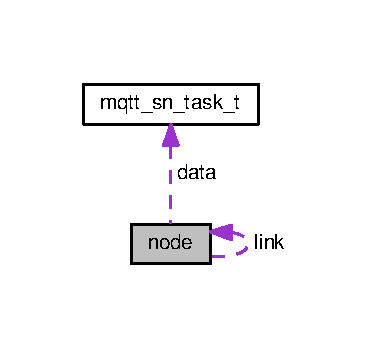
\includegraphics[width=178pt]{structnode__coll__graph}
\end{center}
\end{figure}
\subsection*{Campos de Dados}
\begin{DoxyCompactItemize}
\item 
\hypertarget{structnode_a2a4aa9e422389a8d7a97309a99143ce2}{\hyperlink{structmqtt__sn__task__t}{mqtt\+\_\+sn\+\_\+task\+\_\+t} {\bfseries data}}\label{structnode_a2a4aa9e422389a8d7a97309a99143ce2}

\item 
\hypertarget{structnode_ae20eb3a9a05750fd84dd04b48a8940c3}{struct \hyperlink{structnode}{node} $\ast$ {\bfseries link}}\label{structnode_ae20eb3a9a05750fd84dd04b48a8940c3}

\end{DoxyCompactItemize}


\subsection{Descrição detalhada}
Estrutura de fila M\+Q\+T\+T-\/\+S\+N. 

A documentação para esta estrutura foi gerada a partir do seguinte ficheiro\+:\begin{DoxyCompactItemize}
\item 
\hyperlink{mqtt__sn_8h}{mqtt\+\_\+sn.\+h}\end{DoxyCompactItemize}

\hypertarget{structpublish__packet__t}{\section{Referência à estrutura publish\+\_\+packet\+\_\+t}
\label{structpublish__packet__t}\index{publish\+\_\+packet\+\_\+t@{publish\+\_\+packet\+\_\+t}}
}


estruturas para o bind de topic e short topic id  




{\ttfamily \#include $<$mqtt\+\_\+sn.\+h$>$}

\subsection*{Campos de Dados}
\begin{DoxyCompactItemize}
\item 
\hypertarget{structpublish__packet__t_ab2b3adeb2a67e656ff030b56727fd0ac}{uint8\+\_\+t {\bfseries length}}\label{structpublish__packet__t_ab2b3adeb2a67e656ff030b56727fd0ac}

\item 
\hypertarget{structpublish__packet__t_a1d127017fb298b889f4ba24752d08b8e}{uint8\+\_\+t {\bfseries type}}\label{structpublish__packet__t_a1d127017fb298b889f4ba24752d08b8e}

\item 
\hypertarget{structpublish__packet__t_aa2585d779da0ab21273a8d92de9a0ebe}{uint8\+\_\+t {\bfseries flags}}\label{structpublish__packet__t_aa2585d779da0ab21273a8d92de9a0ebe}

\item 
\hypertarget{structpublish__packet__t_ad562f54acc5597130e0710c356963dff}{uint16\+\_\+t {\bfseries topic\+\_\+id}}\label{structpublish__packet__t_ad562f54acc5597130e0710c356963dff}

\item 
\hypertarget{structpublish__packet__t_aa9c217c6e58cdb2408e2ffbe9425289d}{uint16\+\_\+t {\bfseries message\+\_\+id}}\label{structpublish__packet__t_aa9c217c6e58cdb2408e2ffbe9425289d}

\item 
\hypertarget{structpublish__packet__t_a20288f8717064f4e815c8d57b5fdec41}{char {\bfseries data} \mbox{[}M\+Q\+T\+T\+\_\+\+S\+N\+\_\+\+M\+A\+X\+\_\+\+P\+A\+C\+K\+E\+T\+\_\+\+L\+E\+N\+G\+T\+H-\/7\mbox{]}}\label{structpublish__packet__t_a20288f8717064f4e815c8d57b5fdec41}

\end{DoxyCompactItemize}


\subsection{Descrição detalhada}
estruturas para o bind de topic e short topic id 

Estrutura de pacote do tipo P\+U\+B\+L\+I\+S\+H Identificador da tarefa 

A documentação para esta estrutura foi gerada a partir do seguinte ficheiro\+:\begin{DoxyCompactItemize}
\item 
\hyperlink{mqtt__sn_8h}{mqtt\+\_\+sn.\+h}\end{DoxyCompactItemize}

\hypertarget{structregister__packet__t}{\section{Referência à estrutura register\+\_\+packet\+\_\+t}
\label{structregister__packet__t}\index{register\+\_\+packet\+\_\+t@{register\+\_\+packet\+\_\+t}}
}
\subsection*{Atributos Públicos}
\begin{DoxyCompactItemize}
\item 
\hypertarget{structregister__packet__t_a24462876cab1ee115eab12d1f96f605f}{uint8\+\_\+t {\bfseries length}}\label{structregister__packet__t_a24462876cab1ee115eab12d1f96f605f}

\item 
\hypertarget{structregister__packet__t_a89183a1557a1c6422b0e6b9edf022941}{uint8\+\_\+t {\bfseries type}}\label{structregister__packet__t_a89183a1557a1c6422b0e6b9edf022941}

\item 
\hypertarget{structregister__packet__t_a2dd9b7da1b08d944eff685021eaefd26}{uint16\+\_\+t {\bfseries topic\+\_\+id}}\label{structregister__packet__t_a2dd9b7da1b08d944eff685021eaefd26}

\item 
\hypertarget{structregister__packet__t_af84a2324fa1e64ee1eafbd43e3580f4b}{uint16\+\_\+t {\bfseries message\+\_\+id}}\label{structregister__packet__t_af84a2324fa1e64ee1eafbd43e3580f4b}

\item 
\hypertarget{structregister__packet__t_a10223e5325f38eb2da99e06017220cb9}{char {\bfseries topic\+\_\+name} \mbox{[}M\+Q\+T\+T\+\_\+\+S\+N\+\_\+\+M\+A\+X\+\_\+\+T\+O\+P\+I\+C\+\_\+\+L\+E\+N\+G\+T\+H\mbox{]}}\label{structregister__packet__t_a10223e5325f38eb2da99e06017220cb9}

\end{DoxyCompactItemize}


A documentação para esta estrutura foi gerada a partir do seguinte ficheiro\+:\begin{DoxyCompactItemize}
\item 
mqtt-\/sn.\+h\end{DoxyCompactItemize}

\chapter{Documentação do ficheiro}
\hypertarget{main__core_8c}{\section{Referência ao ficheiro main\+\_\+core.\+c}
\label{main__core_8c}\index{main\+\_\+core.\+c@{main\+\_\+core.\+c}}
}


Arquivo principal do código fonte da rede mesh 6\+Lo\+W\+P\+A\+N ~\newline
 Para compilar este código, execute o makefile com o target desejado, por exemplo\+: ~\newline
 {\bfseries \char`\"{}make T\+A\+R\+G\+E\+T=srf06-\/cc26xx\char`\"{}} ~\newline
 Caso não reconheça qual o T\+A\+R\+G\+E\+T correto, utiliza o comando ~\newline
 {\bfseries \char`\"{}make targets\char`\"{}} ~\newline
 para listar os tags disponíveis.  


{\ttfamily \#include \char`\"{}contiki.\+h\char`\"{}}\\*
{\ttfamily \#include \char`\"{}lib/random.\+h\char`\"{}}\\*
{\ttfamily \#include \char`\"{}clock.\+h\char`\"{}}\\*
{\ttfamily \#include \char`\"{}sys/ctimer.\+h\char`\"{}}\\*
{\ttfamily \#include \char`\"{}net/ip/uip.\+h\char`\"{}}\\*
{\ttfamily \#include \char`\"{}net/ipv6/uip-\/ds6.\+h\char`\"{}}\\*
{\ttfamily \#include \char`\"{}mqtt\+\_\+sn.\+h\char`\"{}}\\*
{\ttfamily \#include \char`\"{}dev/leds.\+h\char`\"{}}\\*
{\ttfamily \#include \char`\"{}net/rime/rime.\+h\char`\"{}}\\*
{\ttfamily \#include \char`\"{}simple-\/udp.\+h\char`\"{}}\\*
{\ttfamily \#include $<$stdio.\+h$>$}\\*
{\ttfamily \#include $<$string.\+h$>$}\\*
{\ttfamily \#include $<$stdlib.\+h$>$}\\*
Diagrama de dependências de inclusão para main\+\_\+core.\+c\+:\nopagebreak
\begin{figure}[H]
\begin{center}
\leavevmode
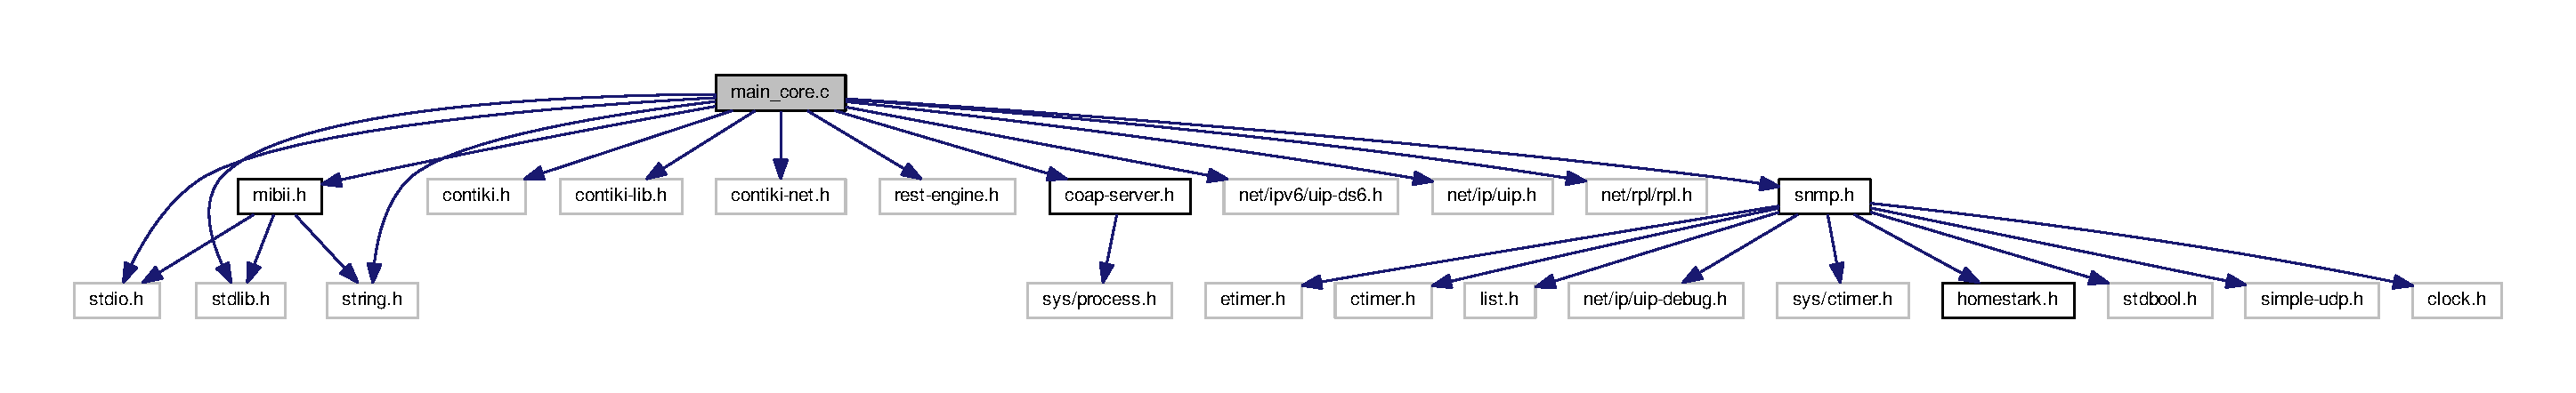
\includegraphics[width=350pt]{main__core_8c__incl}
\end{center}
\end{figure}
\subsection*{Funções}
\begin{DoxyCompactItemize}
\item 
\hypertarget{main__core_8c_a0a43995afea1479f111fbc2e35be0a7c}{void {\bfseries mqtt\+\_\+sn\+\_\+callback} (char $\ast$topic, char $\ast$message)}\label{main__core_8c_a0a43995afea1479f111fbc2e35be0a7c}

\item 
\hypertarget{main__core_8c_a271e0d9822452758a68f6e167c5209f8}{void {\bfseries init\+\_\+broker} (void)}\label{main__core_8c_a271e0d9822452758a68f6e167c5209f8}

\item 
\hypertarget{main__core_8c_a79354dfce54fd0bece29f8d443321b88}{{\bfseries P\+R\+O\+C\+E\+S\+S} (init\+\_\+system\+\_\+process,\char`\"{}\mbox{[}Contiki-\/O\+S\mbox{]} Iniciando sistema operacional\char`\"{})}\label{main__core_8c_a79354dfce54fd0bece29f8d443321b88}

\item 
\hypertarget{main__core_8c_a7683f5bdcb8cfbbb750ce92e76d1b7eb}{{\bfseries P\+R\+O\+C\+E\+S\+S\+\_\+\+T\+H\+R\+E\+A\+D} (init\+\_\+system\+\_\+process, ev, data)}\label{main__core_8c_a7683f5bdcb8cfbbb750ce92e76d1b7eb}

\end{DoxyCompactItemize}
\subsection*{Variáveis}
\begin{DoxyCompactItemize}
\item 
\hypertarget{main__core_8c_a5ca81254b9031056ba22742fb2252fd0}{\hyperlink{structmqtt__sn__con__t}{mqtt\+\_\+sn\+\_\+con\+\_\+t} {\bfseries mqtt\+\_\+sn\+\_\+connection}}\label{main__core_8c_a5ca81254b9031056ba22742fb2252fd0}

\item 
\hypertarget{main__core_8c_ac531a18312af7e29d65ccde0edd8b894}{A\+U\+T\+O\+S\+T\+A\+R\+T\+\_\+\+P\+R\+O\+C\+E\+S\+S\+E\+S \& {\bfseries init\+\_\+system\+\_\+process}}\label{main__core_8c_ac531a18312af7e29d65ccde0edd8b894}

\end{DoxyCompactItemize}


\subsection{Descrição detalhada}
Arquivo principal do código fonte da rede mesh 6\+Lo\+W\+P\+A\+N ~\newline
 Para compilar este código, execute o makefile com o target desejado, por exemplo\+: ~\newline
 {\bfseries \char`\"{}make T\+A\+R\+G\+E\+T=srf06-\/cc26xx\char`\"{}} ~\newline
 Caso não reconheça qual o T\+A\+R\+G\+E\+T correto, utiliza o comando ~\newline
 {\bfseries \char`\"{}make targets\char`\"{}} ~\newline
 para listar os tags disponíveis. 

\begin{DoxyAuthor}{Autor}
Ânderson Ignácio da Silva 
\end{DoxyAuthor}
\begin{DoxyDate}{Data}
19 Ago 2016 
\end{DoxyDate}
\begin{DoxySeeAlso}{Veja também}
\href{http://www.aignacio.com}{\tt http\+://www.\+aignacio.\+com} 
\end{DoxySeeAlso}

\hypertarget{mqtt__sn_8h}{\section{Referência ao ficheiro mqtt\+\_\+sn.\+h}
\label{mqtt__sn_8h}\index{mqtt\+\_\+sn.\+h@{mqtt\+\_\+sn.\+h}}
}


\begin{DoxyVerb}    Conjunto de protótipos e definiçoes do protocolo MQTT-SN
\end{DoxyVerb}
  


{\ttfamily \#include \char`\"{}simple-\/udp.\+h\char`\"{}}\\*
{\ttfamily \#include \char`\"{}clock.\+h\char`\"{}}\\*
{\ttfamily \#include \char`\"{}etimer.\+h\char`\"{}}\\*
{\ttfamily \#include \char`\"{}ctimer.\+h\char`\"{}}\\*
{\ttfamily \#include \char`\"{}list.\+h\char`\"{}}\\*
{\ttfamily \#include \char`\"{}net/ip/uip-\/debug.\+h\char`\"{}}\\*
{\ttfamily \#include \char`\"{}sys/ctimer.\+h\char`\"{}}\\*
{\ttfamily \#include $<$stdbool.\+h$>$}\\*
Diagrama de dependências de inclusão para mqtt\+\_\+sn.\+h\+:\nopagebreak
\begin{figure}[H]
\begin{center}
\leavevmode
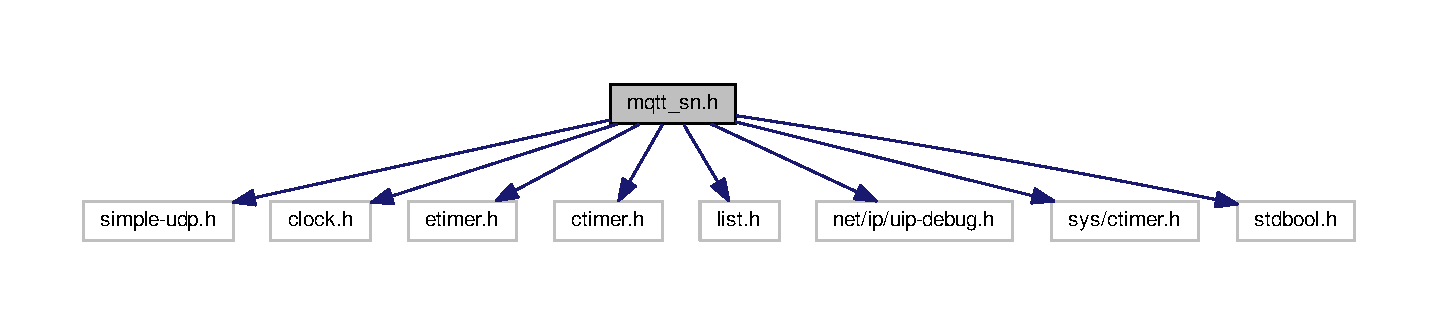
\includegraphics[width=350pt]{mqtt__sn_8h__incl}
\end{center}
\end{figure}
Este grafo mostra quais são os ficheiros que incluem directamente ou indirectamente este ficheiro\+:\nopagebreak
\begin{figure}[H]
\begin{center}
\leavevmode
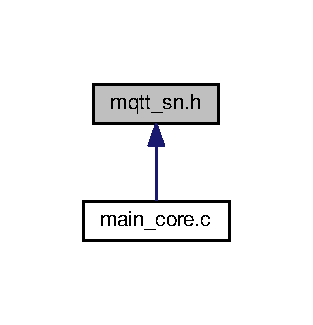
\includegraphics[width=150pt]{mqtt__sn_8h__dep__incl}
\end{center}
\end{figure}
\subsection*{Estruturas de Dados}
\begin{DoxyCompactItemize}
\item 
struct \hyperlink{structpublish__packet__t}{publish\+\_\+packet\+\_\+t}
\begin{DoxyCompactList}\small\item\em estruturas para o bind de topic e short topic id \end{DoxyCompactList}\item 
struct \hyperlink{structmqtt__sn__task__t}{mqtt\+\_\+sn\+\_\+task\+\_\+t}
\begin{DoxyCompactList}\small\item\em Estrutura de tarefa de fila M\+Q\+T\+T-\/\+S\+N. \end{DoxyCompactList}\item 
struct \hyperlink{structnode}{node}
\begin{DoxyCompactList}\small\item\em Estrutura de fila M\+Q\+T\+T-\/\+S\+N. \end{DoxyCompactList}\item 
struct \hyperlink{structconnect__packet__t}{connect\+\_\+packet\+\_\+t}
\begin{DoxyCompactList}\small\item\em Estrutura de pacotes M\+Q\+T\+T-\/\+S\+N do tipo C\+O\+N\+N\+E\+C\+T. \end{DoxyCompactList}\item 
struct \hyperlink{structregister__packet__t}{register\+\_\+packet\+\_\+t}
\begin{DoxyCompactList}\small\item\em Estrutura de pacotes M\+Q\+T\+T-\/\+S\+N do tipo R\+E\+G\+I\+S\+T\+E\+R. \end{DoxyCompactList}\item 
struct \hyperlink{structmqtt__sn__t}{mqtt\+\_\+sn\+\_\+t}
\begin{DoxyCompactList}\small\item\em Estrutura de conexão ao broker M\+Q\+T\+T-\/\+S\+N. \end{DoxyCompactList}\end{DoxyCompactItemize}
\subsection*{Macros}
\begin{DoxyCompactItemize}
\item 
\hypertarget{mqtt__sn_8h_a2949e816367fa801d4015f596cf2925a}{\#define {\bfseries D\+E\+B\+U\+G\+\_\+\+M\+Q\+T\+T\+\_\+\+S\+N}}\label{mqtt__sn_8h_a2949e816367fa801d4015f596cf2925a}

\item 
\hypertarget{mqtt__sn_8h_a7871b41b94f3b5aac9e79ad353903ae7}{\#define {\bfseries D\+E\+B\+U\+G\+\_\+\+O\+S}}\label{mqtt__sn_8h_a7871b41b94f3b5aac9e79ad353903ae7}

\item 
\hypertarget{mqtt__sn_8h_a2308ff2469d9ca327d83e76ddc5e4b9f}{\#define {\bfseries debug\+\_\+logic}(fmt,...)}\label{mqtt__sn_8h_a2308ff2469d9ca327d83e76ddc5e4b9f}

\item 
\hypertarget{mqtt__sn_8h_a4414818dcd874c17a091c7a4d9f9ed37}{\#define {\bfseries debug\+\_\+os}(fmt, args...)~printf(\char`\"{}\textbackslash{}n\mbox{[}H\+O\+M\+E\+S\+T\+A\+R\+K\mbox{]} \char`\"{}fmt, \#\#args)}\label{mqtt__sn_8h_a4414818dcd874c17a091c7a4d9f9ed37}

\item 
\hypertarget{mqtt__sn_8h_ae3e2de92bfa1195fcee6b320e7445986}{\#define {\bfseries debug\+\_\+mqtt}(fmt, args...)~printf(\char`\"{}\textbackslash{}n\mbox{[}M\+Q\+T\+T-\/S\+N\mbox{]} \char`\"{}fmt, \#\#args)}\label{mqtt__sn_8h_ae3e2de92bfa1195fcee6b320e7445986}

\item 
\hypertarget{mqtt__sn_8h_a0d5347618ab59b9090d2d4dfcaf37395}{\#define {\bfseries debug\+\_\+udp}(fmt,...)}\label{mqtt__sn_8h_a0d5347618ab59b9090d2d4dfcaf37395}

\item 
\hypertarget{mqtt__sn_8h_ac6620fe642df6fedae5da980e3cc1685}{\#define {\bfseries M\+Q\+T\+T\+\_\+\+S\+N\+\_\+\+M\+A\+X\+\_\+\+P\+A\+C\+K\+E\+T\+\_\+\+L\+E\+N\+G\+T\+H}~(255)}\label{mqtt__sn_8h_ac6620fe642df6fedae5da980e3cc1685}

\item 
\hypertarget{mqtt__sn_8h_a3dccee9ebffc9265d5c3cd3107ca601b}{\#define {\bfseries M\+Q\+T\+T\+\_\+\+S\+N\+\_\+\+M\+A\+X\+\_\+\+T\+O\+P\+I\+C\+\_\+\+L\+E\+N\+G\+T\+H}~(M\+Q\+T\+T\+\_\+\+S\+N\+\_\+\+M\+A\+X\+\_\+\+P\+A\+C\+K\+E\+T\+\_\+\+L\+E\+N\+G\+T\+H-\/6)}\label{mqtt__sn_8h_a3dccee9ebffc9265d5c3cd3107ca601b}

\item 
\hypertarget{mqtt__sn_8h_a064185df38354c8d31cba8f173a8b39f}{\#define {\bfseries M\+Q\+T\+T\+\_\+\+S\+N\+\_\+\+T\+Y\+P\+E\+\_\+\+A\+D\+V\+E\+R\+T\+I\+S\+E}~(0x00)}\label{mqtt__sn_8h_a064185df38354c8d31cba8f173a8b39f}

\item 
\hypertarget{mqtt__sn_8h_a8170ee7211bec9249606010e8af4765d}{\#define {\bfseries M\+Q\+T\+T\+\_\+\+S\+N\+\_\+\+T\+Y\+P\+E\+\_\+\+S\+E\+A\+R\+C\+H\+G\+W}~(0x01)}\label{mqtt__sn_8h_a8170ee7211bec9249606010e8af4765d}

\item 
\hypertarget{mqtt__sn_8h_a5be35929c3e372b4a2fed0e133be0e92}{\#define {\bfseries M\+Q\+T\+T\+\_\+\+S\+N\+\_\+\+T\+Y\+P\+E\+\_\+\+G\+W\+I\+N\+F\+O}~(0x02)}\label{mqtt__sn_8h_a5be35929c3e372b4a2fed0e133be0e92}

\item 
\hypertarget{mqtt__sn_8h_a0ad512804838d2ba709e82ffb010d991}{\#define {\bfseries M\+Q\+T\+T\+\_\+\+S\+N\+\_\+\+T\+Y\+P\+E\+\_\+\+C\+O\+N\+N\+E\+C\+T}~(0x04)}\label{mqtt__sn_8h_a0ad512804838d2ba709e82ffb010d991}

\item 
\hypertarget{mqtt__sn_8h_ac4469be7c31731176bfa8c5bd38f3a58}{\#define {\bfseries M\+Q\+T\+T\+\_\+\+S\+N\+\_\+\+T\+Y\+P\+E\+\_\+\+C\+O\+N\+N\+A\+C\+K}~(0x05)}\label{mqtt__sn_8h_ac4469be7c31731176bfa8c5bd38f3a58}

\item 
\hypertarget{mqtt__sn_8h_a914fff9b2b9e7c08d6b732599f0cf348}{\#define {\bfseries M\+Q\+T\+T\+\_\+\+S\+N\+\_\+\+T\+Y\+P\+E\+\_\+\+W\+I\+L\+L\+T\+O\+P\+I\+C\+R\+E\+Q}~(0x06)}\label{mqtt__sn_8h_a914fff9b2b9e7c08d6b732599f0cf348}

\item 
\hypertarget{mqtt__sn_8h_a95c657f75f0f02a093b8623a50dc0af8}{\#define {\bfseries M\+Q\+T\+T\+\_\+\+S\+N\+\_\+\+T\+Y\+P\+E\+\_\+\+W\+I\+L\+L\+T\+O\+P\+I\+C}~(0x07)}\label{mqtt__sn_8h_a95c657f75f0f02a093b8623a50dc0af8}

\item 
\hypertarget{mqtt__sn_8h_aefa36203de4d9ff51372abd51fa6521a}{\#define {\bfseries M\+Q\+T\+T\+\_\+\+S\+N\+\_\+\+T\+Y\+P\+E\+\_\+\+W\+I\+L\+L\+M\+S\+G\+R\+E\+Q}~(0x08)}\label{mqtt__sn_8h_aefa36203de4d9ff51372abd51fa6521a}

\item 
\hypertarget{mqtt__sn_8h_a0ab12c9559a2419e1c88080fa3c594c0}{\#define {\bfseries M\+Q\+T\+T\+\_\+\+S\+N\+\_\+\+T\+Y\+P\+E\+\_\+\+W\+I\+L\+L\+M\+S\+G}~(0x09)}\label{mqtt__sn_8h_a0ab12c9559a2419e1c88080fa3c594c0}

\item 
\hypertarget{mqtt__sn_8h_a742472508835bbeab8a22d6294f34e8f}{\#define {\bfseries M\+Q\+T\+T\+\_\+\+S\+N\+\_\+\+T\+Y\+P\+E\+\_\+\+R\+E\+G\+I\+S\+T\+E\+R}~(0x0\+A)}\label{mqtt__sn_8h_a742472508835bbeab8a22d6294f34e8f}

\item 
\hypertarget{mqtt__sn_8h_ab600be8ae75c06a49cc89d0f7255ac12}{\#define {\bfseries M\+Q\+T\+T\+\_\+\+S\+N\+\_\+\+T\+Y\+P\+E\+\_\+\+R\+E\+G\+A\+C\+K}~(0x0\+B)}\label{mqtt__sn_8h_ab600be8ae75c06a49cc89d0f7255ac12}

\item 
\hypertarget{mqtt__sn_8h_a1c34c285be401165ca3b9ef1c9180354}{\#define {\bfseries M\+Q\+T\+T\+\_\+\+S\+N\+\_\+\+T\+Y\+P\+E\+\_\+\+P\+U\+B\+L\+I\+S\+H}~(0x0\+C)}\label{mqtt__sn_8h_a1c34c285be401165ca3b9ef1c9180354}

\item 
\hypertarget{mqtt__sn_8h_a5bc44c53d2905a5242a3b72d44c125b2}{\#define {\bfseries M\+Q\+T\+T\+\_\+\+S\+N\+\_\+\+T\+Y\+P\+E\+\_\+\+P\+U\+B\+A\+C\+K}~(0x0\+D)}\label{mqtt__sn_8h_a5bc44c53d2905a5242a3b72d44c125b2}

\item 
\hypertarget{mqtt__sn_8h_acef39c4b8c3dd36ed4caf90f6a716585}{\#define {\bfseries M\+Q\+T\+T\+\_\+\+S\+N\+\_\+\+T\+Y\+P\+E\+\_\+\+P\+U\+B\+C\+O\+M\+P}~(0x0\+E)}\label{mqtt__sn_8h_acef39c4b8c3dd36ed4caf90f6a716585}

\item 
\hypertarget{mqtt__sn_8h_ac4953c83079abc9804fce7dca7b0a648}{\#define {\bfseries M\+Q\+T\+T\+\_\+\+S\+N\+\_\+\+T\+Y\+P\+E\+\_\+\+P\+U\+B\+R\+E\+C}~(0x0\+F)}\label{mqtt__sn_8h_ac4953c83079abc9804fce7dca7b0a648}

\item 
\hypertarget{mqtt__sn_8h_a74daeb038d5cf996c680fc34b187dfba}{\#define {\bfseries M\+Q\+T\+T\+\_\+\+S\+N\+\_\+\+T\+Y\+P\+E\+\_\+\+P\+U\+B\+R\+E\+L}~(0x10)}\label{mqtt__sn_8h_a74daeb038d5cf996c680fc34b187dfba}

\item 
\hypertarget{mqtt__sn_8h_a1e4f5d7bc584d5ffcda760303ab76904}{\#define {\bfseries M\+Q\+T\+T\+\_\+\+S\+N\+\_\+\+T\+Y\+P\+E\+\_\+\+S\+U\+B\+S\+C\+R\+I\+B\+E}~(0x12)}\label{mqtt__sn_8h_a1e4f5d7bc584d5ffcda760303ab76904}

\item 
\hypertarget{mqtt__sn_8h_a6db4e874ad63924de121a89d4bcd559d}{\#define {\bfseries M\+Q\+T\+T\+\_\+\+S\+N\+\_\+\+T\+Y\+P\+E\+\_\+\+S\+U\+B\+A\+C\+K}~(0x13)}\label{mqtt__sn_8h_a6db4e874ad63924de121a89d4bcd559d}

\item 
\hypertarget{mqtt__sn_8h_a0aaddbe1b0ebd1ece45ada17e618e560}{\#define {\bfseries M\+Q\+T\+T\+\_\+\+S\+N\+\_\+\+T\+Y\+P\+E\+\_\+\+U\+N\+S\+U\+B\+S\+C\+R\+I\+B\+E}~(0x14)}\label{mqtt__sn_8h_a0aaddbe1b0ebd1ece45ada17e618e560}

\item 
\hypertarget{mqtt__sn_8h_a494ee75d7c290823f3738a4d77beea97}{\#define {\bfseries M\+Q\+T\+T\+\_\+\+S\+N\+\_\+\+T\+Y\+P\+E\+\_\+\+U\+N\+S\+U\+B\+A\+C\+K}~(0x15)}\label{mqtt__sn_8h_a494ee75d7c290823f3738a4d77beea97}

\item 
\hypertarget{mqtt__sn_8h_a24c4412f26f5db3dabc57c8511690a7b}{\#define {\bfseries M\+Q\+T\+T\+\_\+\+S\+N\+\_\+\+T\+Y\+P\+E\+\_\+\+P\+I\+N\+G\+R\+E\+Q}~(0x16)}\label{mqtt__sn_8h_a24c4412f26f5db3dabc57c8511690a7b}

\item 
\hypertarget{mqtt__sn_8h_a104849c06dad11e57805341ca6394513}{\#define {\bfseries M\+Q\+T\+T\+\_\+\+S\+N\+\_\+\+T\+Y\+P\+E\+\_\+\+P\+I\+N\+G\+R\+E\+S\+P}~(0x17)}\label{mqtt__sn_8h_a104849c06dad11e57805341ca6394513}

\item 
\hypertarget{mqtt__sn_8h_aeb18a759d020c1443a602636204c6fdd}{\#define {\bfseries M\+Q\+T\+T\+\_\+\+S\+N\+\_\+\+T\+Y\+P\+E\+\_\+\+D\+I\+S\+C\+O\+N\+N\+E\+C\+T}~(0x18)}\label{mqtt__sn_8h_aeb18a759d020c1443a602636204c6fdd}

\item 
\hypertarget{mqtt__sn_8h_ae34bbdc05e79d37cc1f2060a885c3e05}{\#define {\bfseries M\+Q\+T\+T\+\_\+\+S\+N\+\_\+\+T\+Y\+P\+E\+\_\+\+W\+I\+L\+L\+T\+O\+P\+I\+C\+U\+P\+D}~(0x1\+A)}\label{mqtt__sn_8h_ae34bbdc05e79d37cc1f2060a885c3e05}

\item 
\hypertarget{mqtt__sn_8h_a3181a18a9d476f1ca97a1bc935c8b712}{\#define {\bfseries M\+Q\+T\+T\+\_\+\+S\+N\+\_\+\+T\+Y\+P\+E\+\_\+\+W\+I\+L\+L\+T\+O\+P\+I\+C\+R\+E\+S\+P}~(0x1\+B)}\label{mqtt__sn_8h_a3181a18a9d476f1ca97a1bc935c8b712}

\item 
\hypertarget{mqtt__sn_8h_a63c970e654cb17f2a30294a719b11b71}{\#define {\bfseries M\+Q\+T\+T\+\_\+\+S\+N\+\_\+\+T\+Y\+P\+E\+\_\+\+W\+I\+L\+L\+M\+S\+G\+U\+P\+D}~(0x1\+C)}\label{mqtt__sn_8h_a63c970e654cb17f2a30294a719b11b71}

\item 
\hypertarget{mqtt__sn_8h_a855273768c5808acc67a07b8c4b6f5fa}{\#define {\bfseries M\+Q\+T\+T\+\_\+\+S\+N\+\_\+\+T\+Y\+P\+E\+\_\+\+W\+I\+L\+L\+M\+S\+G\+R\+E\+S\+P}~(0x1\+D)}\label{mqtt__sn_8h_a855273768c5808acc67a07b8c4b6f5fa}

\item 
\hypertarget{mqtt__sn_8h_a206c51c6b01cdf9347809ebfc03caaef}{\#define {\bfseries M\+Q\+T\+T\+\_\+\+S\+N\+\_\+\+T\+O\+P\+I\+C\+\_\+\+T\+Y\+P\+E\+\_\+\+N\+O\+R\+M\+A\+L}~(0x00)}\label{mqtt__sn_8h_a206c51c6b01cdf9347809ebfc03caaef}

\item 
\hypertarget{mqtt__sn_8h_a655ae15e8e7734cedf42fab6eb3610b5}{\#define {\bfseries M\+Q\+T\+T\+\_\+\+S\+N\+\_\+\+T\+O\+P\+I\+C\+\_\+\+T\+Y\+P\+E\+\_\+\+P\+R\+E\+D\+E\+F\+I\+N\+E\+D}~(0x01)}\label{mqtt__sn_8h_a655ae15e8e7734cedf42fab6eb3610b5}

\item 
\hypertarget{mqtt__sn_8h_aa17c2076a81b61d2719199521563d1c5}{\#define {\bfseries M\+Q\+T\+T\+\_\+\+S\+N\+\_\+\+T\+O\+P\+I\+C\+\_\+\+T\+Y\+P\+E\+\_\+\+S\+H\+O\+R\+T}~(0x02)}\label{mqtt__sn_8h_aa17c2076a81b61d2719199521563d1c5}

\item 
\hypertarget{mqtt__sn_8h_a2d49bf6469a7864f24a537f059ee0612}{\#define {\bfseries M\+Q\+T\+T\+\_\+\+S\+N\+\_\+\+F\+L\+A\+G\+\_\+\+D\+U\+P}~(0x1 $<$$<$ 7)}\label{mqtt__sn_8h_a2d49bf6469a7864f24a537f059ee0612}

\item 
\hypertarget{mqtt__sn_8h_a37b57822f47fbb4ba1639e5be988c437}{\#define {\bfseries M\+Q\+T\+T\+\_\+\+S\+N\+\_\+\+F\+L\+A\+G\+\_\+\+Q\+O\+S\+\_\+0}~(0x0 $<$$<$ 5)}\label{mqtt__sn_8h_a37b57822f47fbb4ba1639e5be988c437}

\item 
\hypertarget{mqtt__sn_8h_a6d04b90ba54b58e08caa593a84105f21}{\#define {\bfseries M\+Q\+T\+T\+\_\+\+S\+N\+\_\+\+F\+L\+A\+G\+\_\+\+Q\+O\+S\+\_\+1}~(0x1 $<$$<$ 5)}\label{mqtt__sn_8h_a6d04b90ba54b58e08caa593a84105f21}

\item 
\hypertarget{mqtt__sn_8h_a953eaf715ee6055e9f119950be8d7399}{\#define {\bfseries M\+Q\+T\+T\+\_\+\+S\+N\+\_\+\+F\+L\+A\+G\+\_\+\+Q\+O\+S\+\_\+2}~(0x2 $<$$<$ 5)}\label{mqtt__sn_8h_a953eaf715ee6055e9f119950be8d7399}

\item 
\hypertarget{mqtt__sn_8h_a8095eefa31299b606b4ba8bbbcb00195}{\#define {\bfseries M\+Q\+T\+T\+\_\+\+S\+N\+\_\+\+F\+L\+A\+G\+\_\+\+Q\+O\+S\+\_\+\+N1}~(0x3 $<$$<$ 5)}\label{mqtt__sn_8h_a8095eefa31299b606b4ba8bbbcb00195}

\item 
\hypertarget{mqtt__sn_8h_a45271b87fd548295bc4c86c225fc648e}{\#define {\bfseries M\+Q\+T\+T\+\_\+\+S\+N\+\_\+\+F\+L\+A\+G\+\_\+\+R\+E\+T\+A\+I\+N}~(0x1 $<$$<$ 4)}\label{mqtt__sn_8h_a45271b87fd548295bc4c86c225fc648e}

\item 
\hypertarget{mqtt__sn_8h_a8e3f7578e0fef59224e365cef8613f8e}{\#define {\bfseries M\+Q\+T\+T\+\_\+\+S\+N\+\_\+\+F\+L\+A\+G\+\_\+\+W\+I\+L\+L}~(0x1 $<$$<$ 3)}\label{mqtt__sn_8h_a8e3f7578e0fef59224e365cef8613f8e}

\item 
\hypertarget{mqtt__sn_8h_a842ab1c7124c0b63f62ed3283dafbe06}{\#define {\bfseries M\+Q\+T\+T\+\_\+\+S\+N\+\_\+\+F\+L\+A\+G\+\_\+\+C\+L\+E\+A\+N}~(0x1 $<$$<$ 2)}\label{mqtt__sn_8h_a842ab1c7124c0b63f62ed3283dafbe06}

\item 
\hypertarget{mqtt__sn_8h_a0066dd4afeef507b2e8f5ac01f71ea37}{\#define {\bfseries M\+Q\+T\+T\+\_\+\+S\+N\+\_\+\+P\+R\+O\+T\+O\+C\+O\+L\+\_\+\+I\+D}~(0x01)}\label{mqtt__sn_8h_a0066dd4afeef507b2e8f5ac01f71ea37}

\item 
\hypertarget{mqtt__sn_8h_a43005b6b1934800f67a6d169c779c92b}{\#define {\bfseries A\+C\+C\+E\+P\+T\+E\+D}~0x00}\label{mqtt__sn_8h_a43005b6b1934800f67a6d169c779c92b}

\item 
\hypertarget{mqtt__sn_8h_a9b2b214d1ddb0f617efdd26ccc91def4}{\#define {\bfseries R\+E\+J\+E\+C\+T\+E\+D\+\_\+\+C\+O\+N\+G\+E\+S\+T\+I\+O\+N}~0x01}\label{mqtt__sn_8h_a9b2b214d1ddb0f617efdd26ccc91def4}

\item 
\hypertarget{mqtt__sn_8h_a9b548f6c60530b07c9b9f5ef5b1ac8b9}{\#define {\bfseries R\+E\+J\+E\+C\+T\+E\+D\+\_\+\+I\+N\+V\+A\+L\+I\+D\+\_\+\+T\+O\+P\+I\+C\+\_\+\+I\+D}~0x02}\label{mqtt__sn_8h_a9b548f6c60530b07c9b9f5ef5b1ac8b9}

\item 
\hypertarget{mqtt__sn_8h_a93af4e6b658c4823ae9603b86bb7c64a}{\#define {\bfseries R\+E\+J\+E\+C\+T\+E\+D\+\_\+\+N\+O\+T\+\_\+\+S\+U\+P\+P\+O\+R\+T\+E\+D}~0x03}\label{mqtt__sn_8h_a93af4e6b658c4823ae9603b86bb7c64a}

\item 
\hypertarget{mqtt__sn_8h_a47da8d46176b160b0db00fe221725d4c}{\#define {\bfseries M\+Q\+T\+T\+\_\+\+S\+N\+\_\+\+T\+I\+M\+E\+O\+U\+T}~C\+L\+O\+C\+K\+\_\+\+S\+E\+C\+O\+N\+D}\label{mqtt__sn_8h_a47da8d46176b160b0db00fe221725d4c}

\item 
\hypertarget{mqtt__sn_8h_aad5ac7de3008d8fa37447193aebc31e2}{\#define {\bfseries M\+Q\+T\+T\+\_\+\+S\+N\+\_\+\+R\+E\+T\+R\+Y}~5}\label{mqtt__sn_8h_aad5ac7de3008d8fa37447193aebc31e2}

\item 
\hypertarget{mqtt__sn_8h_a45ab5881e190d570f3784e50be2cce65}{\#define {\bfseries M\+A\+X\+\_\+\+Q\+U\+E\+U\+E\+\_\+\+M\+Q\+T\+T\+\_\+\+S\+N}~100}\label{mqtt__sn_8h_a45ab5881e190d570f3784e50be2cce65}

\item 
\hypertarget{mqtt__sn_8h_a5ed98e8fc00194886ebc14d25540f81b}{\#define {\bfseries M\+A\+X\+\_\+\+T\+O\+P\+I\+C\+\_\+\+U\+S\+E\+D}~10}\label{mqtt__sn_8h_a5ed98e8fc00194886ebc14d25540f81b}

\end{DoxyCompactItemize}
\subsection*{Definições de tipos}
\begin{DoxyCompactItemize}
\item 
\hypertarget{mqtt__sn_8h_add91ba4199db8665b9b9fc56fc6783a6}{typedef enum \hyperlink{mqtt__sn_8h_a754c1055b4431040415cf01b39caaa98}{resp\+\_\+con} \hyperlink{mqtt__sn_8h_add91ba4199db8665b9b9fc56fc6783a6}{resp\+\_\+con\+\_\+t}}\label{mqtt__sn_8h_add91ba4199db8665b9b9fc56fc6783a6}

\begin{DoxyCompactList}\small\item\em Tipo de erros de funções. \end{DoxyCompactList}\item 
\hypertarget{mqtt__sn_8h_aab2bca192b63f37bf4847be3686bca75}{typedef enum \hyperlink{mqtt__sn_8h_a14f5db3d1cf62de306c396a70251022c}{mqtt\+\_\+sn\+\_\+status} \hyperlink{mqtt__sn_8h_aab2bca192b63f37bf4847be3686bca75}{mqtt\+\_\+sn\+\_\+status\+\_\+t}}\label{mqtt__sn_8h_aab2bca192b63f37bf4847be3686bca75}

\begin{DoxyCompactList}\small\item\em Estados da A\+S\+M do M\+Q\+T\+T-\/\+S\+N. \end{DoxyCompactList}\item 
\hypertarget{mqtt__sn_8h_aed5d1362b055e38731f5c556a102fc36}{typedef enum \hyperlink{mqtt__sn_8h_a66c59ab6d5a32b88c55f35d6ffc3f0d6}{mqtt\+\_\+sn\+\_\+status\+\_\+2} \hyperlink{mqtt__sn_8h_aed5d1362b055e38731f5c556a102fc36}{mqtt\+\_\+sn\+\_\+messages\+\_\+status\+\_\+t}}\label{mqtt__sn_8h_aed5d1362b055e38731f5c556a102fc36}

\begin{DoxyCompactList}\small\item\em Estados da A\+S\+M do M\+Q\+T\+T-\/\+S\+N depois de conectado ao broker. \end{DoxyCompactList}\end{DoxyCompactItemize}
\subsection*{Enumerações}
\begin{DoxyCompactItemize}
\item 
enum \hyperlink{mqtt__sn_8h_a754c1055b4431040415cf01b39caaa98}{resp\+\_\+con} \{ \hyperlink{mqtt__sn_8h_a754c1055b4431040415cf01b39caaa98ac6ae922662cbaf7958eb387bfd6fe4da}{F\+A\+I\+L\+\_\+\+C\+O\+N}, 
\hyperlink{mqtt__sn_8h_a754c1055b4431040415cf01b39caaa98ae7b7a388c90c2c5428cced225760885f}{S\+U\+C\+C\+E\+S\+S\+\_\+\+C\+O\+N}
 \}
\item 
enum \hyperlink{mqtt__sn_8h_a14f5db3d1cf62de306c396a70251022c}{mqtt\+\_\+sn\+\_\+status} \{ \\*
\hyperlink{mqtt__sn_8h_a14f5db3d1cf62de306c396a70251022ca8b9b93d8c6ff288b5122906cbd74793e}{M\+Q\+T\+T\+S\+N\+\_\+\+D\+I\+S\+C\+O\+N\+N\+E\+C\+T\+E\+D}, 
\hyperlink{mqtt__sn_8h_a14f5db3d1cf62de306c396a70251022ca838970c34c36be6d92ef83b92d66225b}{M\+Q\+T\+T\+S\+N\+\_\+\+W\+A\+I\+T\+I\+N\+G\+\_\+\+C\+O\+N\+N\+A\+C\+K}, 
\hyperlink{mqtt__sn_8h_a14f5db3d1cf62de306c396a70251022caed256d36bd284e414f365c5ba56cf563}{M\+Q\+T\+T\+S\+N\+\_\+\+C\+O\+N\+N\+E\+C\+T\+I\+O\+N\+\_\+\+F\+A\+I\+L\+E\+D}, 
\hyperlink{mqtt__sn_8h_a14f5db3d1cf62de306c396a70251022cac196945518fdb65f40760e324458a955}{M\+Q\+T\+T\+S\+N\+\_\+\+C\+O\+N\+N\+E\+C\+T\+E\+D}, 
\\*
\hyperlink{mqtt__sn_8h_a14f5db3d1cf62de306c396a70251022ca1e692a063bcd40c0615a2e6516cfc68d}{M\+Q\+T\+T\+S\+N\+\_\+\+I\+D\+D\+L\+E}
 \}
\item 
enum \hyperlink{mqtt__sn_8h_a66c59ab6d5a32b88c55f35d6ffc3f0d6}{mqtt\+\_\+sn\+\_\+status\+\_\+2} \{ \\*
\hyperlink{mqtt__sn_8h_a66c59ab6d5a32b88c55f35d6ffc3f0d6a1fe0503c5c2768076758893cefd1d46e}{M\+Q\+T\+T\+S\+N\+\_\+\+W\+A\+I\+T\+I\+N\+G\+\_\+\+R\+E\+G\+A\+C\+K}, 
\hyperlink{mqtt__sn_8h_a66c59ab6d5a32b88c55f35d6ffc3f0d6a5c12b36470411b7ed7a890f8916c4db2}{M\+Q\+T\+T\+S\+N\+\_\+\+W\+A\+I\+T\+I\+N\+G\+\_\+\+P\+U\+B\+A\+C\+K}, 
\hyperlink{mqtt__sn_8h_a66c59ab6d5a32b88c55f35d6ffc3f0d6a459f16ecc3340a5e6e3f61c772d68a6f}{M\+Q\+T\+T\+S\+N\+\_\+\+W\+A\+I\+T\+I\+N\+G\+\_\+\+S\+U\+B\+A\+C\+K}, 
{\bfseries I\+D\+D\+L\+E}, 
\\*
{\bfseries M\+Q\+T\+T\+S\+N\+\_\+\+P\+U\+B\+\_\+\+R\+E\+Q}, 
{\bfseries M\+Q\+T\+T\+S\+N\+\_\+\+S\+U\+B\+\_\+\+R\+E\+Q}, 
{\bfseries M\+Q\+T\+T\+S\+N\+\_\+\+R\+E\+G\+\_\+\+R\+E\+Q}
 \}
\end{DoxyCompactItemize}
\subsection*{Funções}
\begin{DoxyCompactItemize}
\item 
\hyperlink{mqtt__sn_8h_add91ba4199db8665b9b9fc56fc6783a6}{resp\+\_\+con\+\_\+t} \hyperlink{mqtt__sn_8h_a575514d0f0fd3b6c5c4a2c75e604bf79}{mqtt\+\_\+sn\+\_\+insert\+\_\+queue} (\hyperlink{structmqtt__sn__task__t}{mqtt\+\_\+sn\+\_\+task\+\_\+t} new)
\begin{DoxyCompactList}\small\item\em Insere uma tarefa na fila. \end{DoxyCompactList}\item 
void \hyperlink{mqtt__sn_8h_ad0a729c99366dad086be6be954e71f2c}{mqtt\+\_\+sn\+\_\+delete\+\_\+queue} ()
\begin{DoxyCompactList}\small\item\em Remove o elemento mais próximo de ser processado. \end{DoxyCompactList}\item 
void \hyperlink{mqtt__sn_8h_a71004d5b7e8b1add14024102d8d62042}{mqtt\+\_\+sn\+\_\+check\+\_\+queue} ()
\begin{DoxyCompactList}\small\item\em Lista as tarefas da fila. \end{DoxyCompactList}\item 
\hyperlink{mqtt__sn_8h_add91ba4199db8665b9b9fc56fc6783a6}{resp\+\_\+con\+\_\+t} \hyperlink{mqtt__sn_8h_a172afa34fe10ad1ee4ffc0d226b35b4d}{mqtt\+\_\+sn\+\_\+check\+\_\+rc} (uint8\+\_\+t rc)
\begin{DoxyCompactList}\small\item\em Envia requisição de conexão ao broker M\+Q\+T\+T-\/\+S\+N. \end{DoxyCompactList}\item 
void \hyperlink{mqtt__sn_8h_ac1ce35580b749c06730f04f6e56cbee7}{mqtt\+\_\+sn\+\_\+connect\+\_\+request} (void)
\begin{DoxyCompactList}\small\item\em Envia requisição de conexão ao broker M\+Q\+T\+T-\/\+S\+N. \end{DoxyCompactList}\item 
void \hyperlink{mqtt__sn_8h_add57b9872ddb83d265d498a7dd5cba7d}{mqtt\+\_\+sn\+\_\+state\+\_\+ctrl} (void $\ast$ptr)
\begin{DoxyCompactList}\small\item\em Controla o estado da conexão M\+Q\+T\+T-\/\+S\+N. \end{DoxyCompactList}\item 
void \hyperlink{mqtt__sn_8h_af9146fa082fe2bc6612fb13dbb20ed36}{mqtt\+\_\+sn\+\_\+recv\+\_\+parser} (const uint8\+\_\+t $\ast$data)
\begin{DoxyCompactList}\small\item\em Realiza o parsing das mensagens U\+D\+P recebidas. \end{DoxyCompactList}\item 
\hyperlink{mqtt__sn_8h_add91ba4199db8665b9b9fc56fc6783a6}{resp\+\_\+con\+\_\+t} \hyperlink{mqtt__sn_8h_a707413f00362e05c733c2b2f5f3c138c}{mqtt\+\_\+sn\+\_\+create\+\_\+sck} (\hyperlink{structmqtt__sn__t}{mqtt\+\_\+sn\+\_\+t} mqtt\+\_\+sn\+\_\+connection, char $\ast$topics\mbox{[}$\,$\mbox{]}, size\+\_\+t topic\+\_\+len)
\begin{DoxyCompactList}\small\item\em Inicia conexão ao broker U\+D\+P. \end{DoxyCompactList}\item 
\hyperlink{mqtt__sn_8h_add91ba4199db8665b9b9fc56fc6783a6}{resp\+\_\+con\+\_\+t} \hyperlink{mqtt__sn_8h_a2804f776c1813e59dd2927d17e6a10c2}{mqtt\+\_\+sn\+\_\+reg\+\_\+task} (char $\ast$topic\+\_\+name)
\begin{DoxyCompactList}\small\item\em Registro de tópicos M\+Q\+T\+T-\/\+S\+N. \end{DoxyCompactList}\item 
void \hyperlink{mqtt__sn_8h_a2b9f8f5b6189f0242ae7e6908775d615}{mqtt\+\_\+main\+\_\+connected} (void)
\begin{DoxyCompactList}\small\item\em Máquina de estados principal do M\+Q\+T\+T-\/\+S\+N. \end{DoxyCompactList}\item 
\hyperlink{mqtt__sn_8h_add91ba4199db8665b9b9fc56fc6783a6}{resp\+\_\+con\+\_\+t} \hyperlink{mqtt__sn_8h_ae17664af7f894e29743fafdf8bf98f89}{mqtt\+\_\+sn\+\_\+reg\+\_\+send} (void)
\begin{DoxyCompactList}\small\item\em Envio de mensagens ao broker do tipo R\+E\+G\+I\+S\+T\+E\+R. \end{DoxyCompactList}\item 
\hypertarget{mqtt__sn_8h_ac598f98e844bfd5bbdb577099ddf06d1}{void {\bfseries parse\+\_\+mqtt\+\_\+type\+\_\+string} (uint8\+\_\+t type, char $\ast$$\ast$type\+\_\+string)}\label{mqtt__sn_8h_ac598f98e844bfd5bbdb577099ddf06d1}

\item 
\hypertarget{mqtt__sn_8h_a46fe607d1db728d41ed6aec6fee3fc77}{void {\bfseries mqtt\+\_\+sn\+\_\+init} (void)}\label{mqtt__sn_8h_a46fe607d1db728d41ed6aec6fee3fc77}

\end{DoxyCompactItemize}
\subsection*{Variáveis}
\begin{DoxyCompactItemize}
\item 
\hypertarget{mqtt__sn_8h_a47c68c75b7151c412b3e13a0752a3a43}{struct \hyperlink{structnode}{node} $\ast$ {\bfseries mqtt\+\_\+queue\+\_\+first}}\label{mqtt__sn_8h_a47c68c75b7151c412b3e13a0752a3a43}

\item 
\hypertarget{mqtt__sn_8h_a777f6f15b97e834ca56d2b35f55846d0}{struct \hyperlink{structnode}{node} $\ast$ {\bfseries mqtt\+\_\+queue\+\_\+last}}\label{mqtt__sn_8h_a777f6f15b97e834ca56d2b35f55846d0}

\end{DoxyCompactItemize}


\subsection{Descrição detalhada}
\begin{DoxyVerb}    Conjunto de protótipos e definiçoes do protocolo MQTT-SN
\end{DoxyVerb}
 

\begin{DoxyAuthor}{Autor}
Ânderson Ignácio da Silva \href{mailto:anderson@aignacio.com}{\tt anderson@aignacio.\+com} 
\end{DoxyAuthor}


\subsection{Documentação dos valores da enumeração}
\hypertarget{mqtt__sn_8h_a14f5db3d1cf62de306c396a70251022c}{\index{mqtt\+\_\+sn.\+h@{mqtt\+\_\+sn.\+h}!mqtt\+\_\+sn\+\_\+status@{mqtt\+\_\+sn\+\_\+status}}
\index{mqtt\+\_\+sn\+\_\+status@{mqtt\+\_\+sn\+\_\+status}!mqtt\+\_\+sn.\+h@{mqtt\+\_\+sn.\+h}}
\subsubsection[{mqtt\+\_\+sn\+\_\+status}]{\setlength{\rightskip}{0pt plus 5cm}enum {\bf mqtt\+\_\+sn\+\_\+status}}}\label{mqtt__sn_8h_a14f5db3d1cf62de306c396a70251022c}
\begin{Desc}
\item[Valores da enumeração]\par
\begin{description}
\index{M\+Q\+T\+T\+S\+N\+\_\+\+D\+I\+S\+C\+O\+N\+N\+E\+C\+T\+E\+D@{M\+Q\+T\+T\+S\+N\+\_\+\+D\+I\+S\+C\+O\+N\+N\+E\+C\+T\+E\+D}!mqtt\+\_\+sn.\+h@{mqtt\+\_\+sn.\+h}}\index{mqtt\+\_\+sn.\+h@{mqtt\+\_\+sn.\+h}!M\+Q\+T\+T\+S\+N\+\_\+\+D\+I\+S\+C\+O\+N\+N\+E\+C\+T\+E\+D@{M\+Q\+T\+T\+S\+N\+\_\+\+D\+I\+S\+C\+O\+N\+N\+E\+C\+T\+E\+D}}\item[{\em 
\hypertarget{mqtt__sn_8h_a14f5db3d1cf62de306c396a70251022ca8b9b93d8c6ff288b5122906cbd74793e}{M\+Q\+T\+T\+S\+N\+\_\+\+D\+I\+S\+C\+O\+N\+N\+E\+C\+T\+E\+D}\label{mqtt__sn_8h_a14f5db3d1cf62de306c396a70251022ca8b9b93d8c6ff288b5122906cbd74793e}
}]Desconectado do broker M\+Q\+T\+T-\/\+S\+N. \index{M\+Q\+T\+T\+S\+N\+\_\+\+W\+A\+I\+T\+I\+N\+G\+\_\+\+C\+O\+N\+N\+A\+C\+K@{M\+Q\+T\+T\+S\+N\+\_\+\+W\+A\+I\+T\+I\+N\+G\+\_\+\+C\+O\+N\+N\+A\+C\+K}!mqtt\+\_\+sn.\+h@{mqtt\+\_\+sn.\+h}}\index{mqtt\+\_\+sn.\+h@{mqtt\+\_\+sn.\+h}!M\+Q\+T\+T\+S\+N\+\_\+\+W\+A\+I\+T\+I\+N\+G\+\_\+\+C\+O\+N\+N\+A\+C\+K@{M\+Q\+T\+T\+S\+N\+\_\+\+W\+A\+I\+T\+I\+N\+G\+\_\+\+C\+O\+N\+N\+A\+C\+K}}\item[{\em 
\hypertarget{mqtt__sn_8h_a14f5db3d1cf62de306c396a70251022ca838970c34c36be6d92ef83b92d66225b}{M\+Q\+T\+T\+S\+N\+\_\+\+W\+A\+I\+T\+I\+N\+G\+\_\+\+C\+O\+N\+N\+A\+C\+K}\label{mqtt__sn_8h_a14f5db3d1cf62de306c396a70251022ca838970c34c36be6d92ef83b92d66225b}
}]Aguardando C\+O\+N\+N\+A\+C\+K do broker. \index{M\+Q\+T\+T\+S\+N\+\_\+\+C\+O\+N\+N\+E\+C\+T\+I\+O\+N\+\_\+\+F\+A\+I\+L\+E\+D@{M\+Q\+T\+T\+S\+N\+\_\+\+C\+O\+N\+N\+E\+C\+T\+I\+O\+N\+\_\+\+F\+A\+I\+L\+E\+D}!mqtt\+\_\+sn.\+h@{mqtt\+\_\+sn.\+h}}\index{mqtt\+\_\+sn.\+h@{mqtt\+\_\+sn.\+h}!M\+Q\+T\+T\+S\+N\+\_\+\+C\+O\+N\+N\+E\+C\+T\+I\+O\+N\+\_\+\+F\+A\+I\+L\+E\+D@{M\+Q\+T\+T\+S\+N\+\_\+\+C\+O\+N\+N\+E\+C\+T\+I\+O\+N\+\_\+\+F\+A\+I\+L\+E\+D}}\item[{\em 
\hypertarget{mqtt__sn_8h_a14f5db3d1cf62de306c396a70251022caed256d36bd284e414f365c5ba56cf563}{M\+Q\+T\+T\+S\+N\+\_\+\+C\+O\+N\+N\+E\+C\+T\+I\+O\+N\+\_\+\+F\+A\+I\+L\+E\+D}\label{mqtt__sn_8h_a14f5db3d1cf62de306c396a70251022caed256d36bd284e414f365c5ba56cf563}
}]Falha na conexão com o broker M\+Q\+T\+T-\/\+S\+N. \index{M\+Q\+T\+T\+S\+N\+\_\+\+C\+O\+N\+N\+E\+C\+T\+E\+D@{M\+Q\+T\+T\+S\+N\+\_\+\+C\+O\+N\+N\+E\+C\+T\+E\+D}!mqtt\+\_\+sn.\+h@{mqtt\+\_\+sn.\+h}}\index{mqtt\+\_\+sn.\+h@{mqtt\+\_\+sn.\+h}!M\+Q\+T\+T\+S\+N\+\_\+\+C\+O\+N\+N\+E\+C\+T\+E\+D@{M\+Q\+T\+T\+S\+N\+\_\+\+C\+O\+N\+N\+E\+C\+T\+E\+D}}\item[{\em 
\hypertarget{mqtt__sn_8h_a14f5db3d1cf62de306c396a70251022cac196945518fdb65f40760e324458a955}{M\+Q\+T\+T\+S\+N\+\_\+\+C\+O\+N\+N\+E\+C\+T\+E\+D}\label{mqtt__sn_8h_a14f5db3d1cf62de306c396a70251022cac196945518fdb65f40760e324458a955}
}]Conectado ao broker M\+Q\+T\+T-\/\+S\+N. \index{M\+Q\+T\+T\+S\+N\+\_\+\+I\+D\+D\+L\+E@{M\+Q\+T\+T\+S\+N\+\_\+\+I\+D\+D\+L\+E}!mqtt\+\_\+sn.\+h@{mqtt\+\_\+sn.\+h}}\index{mqtt\+\_\+sn.\+h@{mqtt\+\_\+sn.\+h}!M\+Q\+T\+T\+S\+N\+\_\+\+I\+D\+D\+L\+E@{M\+Q\+T\+T\+S\+N\+\_\+\+I\+D\+D\+L\+E}}\item[{\em 
\hypertarget{mqtt__sn_8h_a14f5db3d1cf62de306c396a70251022ca1e692a063bcd40c0615a2e6516cfc68d}{M\+Q\+T\+T\+S\+N\+\_\+\+I\+D\+D\+L\+E}\label{mqtt__sn_8h_a14f5db3d1cf62de306c396a70251022ca1e692a063bcd40c0615a2e6516cfc68d}
}]Estado reservado para conexão ao broker M\+Q\+T\+T-\/\+S\+N. \end{description}
\end{Desc}

\begin{DoxyCode}
230                            \{
231   \hyperlink{mqtt__sn_8h_a14f5db3d1cf62de306c396a70251022ca8b9b93d8c6ff288b5122906cbd74793e}{MQTTSN\_DISCONNECTED},
232   \hyperlink{mqtt__sn_8h_a14f5db3d1cf62de306c396a70251022ca838970c34c36be6d92ef83b92d66225b}{MQTTSN\_WAITING\_CONNACK},
233   \hyperlink{mqtt__sn_8h_a14f5db3d1cf62de306c396a70251022caed256d36bd284e414f365c5ba56cf563}{MQTTSN\_CONNECTION\_FAILED},
234   \hyperlink{mqtt__sn_8h_a14f5db3d1cf62de306c396a70251022cac196945518fdb65f40760e324458a955}{MQTTSN\_CONNECTED},
235   \hyperlink{mqtt__sn_8h_a14f5db3d1cf62de306c396a70251022ca1e692a063bcd40c0615a2e6516cfc68d}{MQTTSN\_IDDLE}
236 \} \hyperlink{mqtt__sn_8h_aab2bca192b63f37bf4847be3686bca75}{mqtt\_sn\_status\_t};
\end{DoxyCode}
\hypertarget{mqtt__sn_8h_a66c59ab6d5a32b88c55f35d6ffc3f0d6}{\index{mqtt\+\_\+sn.\+h@{mqtt\+\_\+sn.\+h}!mqtt\+\_\+sn\+\_\+status\+\_\+2@{mqtt\+\_\+sn\+\_\+status\+\_\+2}}
\index{mqtt\+\_\+sn\+\_\+status\+\_\+2@{mqtt\+\_\+sn\+\_\+status\+\_\+2}!mqtt\+\_\+sn.\+h@{mqtt\+\_\+sn.\+h}}
\subsubsection[{mqtt\+\_\+sn\+\_\+status\+\_\+2}]{\setlength{\rightskip}{0pt plus 5cm}enum {\bf mqtt\+\_\+sn\+\_\+status\+\_\+2}}}\label{mqtt__sn_8h_a66c59ab6d5a32b88c55f35d6ffc3f0d6}
\begin{Desc}
\item[Valores da enumeração]\par
\begin{description}
\index{M\+Q\+T\+T\+S\+N\+\_\+\+W\+A\+I\+T\+I\+N\+G\+\_\+\+R\+E\+G\+A\+C\+K@{M\+Q\+T\+T\+S\+N\+\_\+\+W\+A\+I\+T\+I\+N\+G\+\_\+\+R\+E\+G\+A\+C\+K}!mqtt\+\_\+sn.\+h@{mqtt\+\_\+sn.\+h}}\index{mqtt\+\_\+sn.\+h@{mqtt\+\_\+sn.\+h}!M\+Q\+T\+T\+S\+N\+\_\+\+W\+A\+I\+T\+I\+N\+G\+\_\+\+R\+E\+G\+A\+C\+K@{M\+Q\+T\+T\+S\+N\+\_\+\+W\+A\+I\+T\+I\+N\+G\+\_\+\+R\+E\+G\+A\+C\+K}}\item[{\em 
\hypertarget{mqtt__sn_8h_a66c59ab6d5a32b88c55f35d6ffc3f0d6a1fe0503c5c2768076758893cefd1d46e}{M\+Q\+T\+T\+S\+N\+\_\+\+W\+A\+I\+T\+I\+N\+G\+\_\+\+R\+E\+G\+A\+C\+K}\label{mqtt__sn_8h_a66c59ab6d5a32b88c55f35d6ffc3f0d6a1fe0503c5c2768076758893cefd1d46e}
}]Aguardando R\+E\+G\+A\+C\+K do broker. \index{M\+Q\+T\+T\+S\+N\+\_\+\+W\+A\+I\+T\+I\+N\+G\+\_\+\+P\+U\+B\+A\+C\+K@{M\+Q\+T\+T\+S\+N\+\_\+\+W\+A\+I\+T\+I\+N\+G\+\_\+\+P\+U\+B\+A\+C\+K}!mqtt\+\_\+sn.\+h@{mqtt\+\_\+sn.\+h}}\index{mqtt\+\_\+sn.\+h@{mqtt\+\_\+sn.\+h}!M\+Q\+T\+T\+S\+N\+\_\+\+W\+A\+I\+T\+I\+N\+G\+\_\+\+P\+U\+B\+A\+C\+K@{M\+Q\+T\+T\+S\+N\+\_\+\+W\+A\+I\+T\+I\+N\+G\+\_\+\+P\+U\+B\+A\+C\+K}}\item[{\em 
\hypertarget{mqtt__sn_8h_a66c59ab6d5a32b88c55f35d6ffc3f0d6a5c12b36470411b7ed7a890f8916c4db2}{M\+Q\+T\+T\+S\+N\+\_\+\+W\+A\+I\+T\+I\+N\+G\+\_\+\+P\+U\+B\+A\+C\+K}\label{mqtt__sn_8h_a66c59ab6d5a32b88c55f35d6ffc3f0d6a5c12b36470411b7ed7a890f8916c4db2}
}]Aguardando P\+U\+B\+A\+C\+K do broker. \index{M\+Q\+T\+T\+S\+N\+\_\+\+W\+A\+I\+T\+I\+N\+G\+\_\+\+S\+U\+B\+A\+C\+K@{M\+Q\+T\+T\+S\+N\+\_\+\+W\+A\+I\+T\+I\+N\+G\+\_\+\+S\+U\+B\+A\+C\+K}!mqtt\+\_\+sn.\+h@{mqtt\+\_\+sn.\+h}}\index{mqtt\+\_\+sn.\+h@{mqtt\+\_\+sn.\+h}!M\+Q\+T\+T\+S\+N\+\_\+\+W\+A\+I\+T\+I\+N\+G\+\_\+\+S\+U\+B\+A\+C\+K@{M\+Q\+T\+T\+S\+N\+\_\+\+W\+A\+I\+T\+I\+N\+G\+\_\+\+S\+U\+B\+A\+C\+K}}\item[{\em 
\hypertarget{mqtt__sn_8h_a66c59ab6d5a32b88c55f35d6ffc3f0d6a459f16ecc3340a5e6e3f61c772d68a6f}{M\+Q\+T\+T\+S\+N\+\_\+\+W\+A\+I\+T\+I\+N\+G\+\_\+\+S\+U\+B\+A\+C\+K}\label{mqtt__sn_8h_a66c59ab6d5a32b88c55f35d6ffc3f0d6a459f16ecc3340a5e6e3f61c772d68a6f}
}]Aguardando S\+U\+B\+A\+C\+K do broker. \end{description}
\end{Desc}

\begin{DoxyCode}
249                              \{
250   \hyperlink{mqtt__sn_8h_a66c59ab6d5a32b88c55f35d6ffc3f0d6a1fe0503c5c2768076758893cefd1d46e}{MQTTSN\_WAITING\_REGACK},
251   \hyperlink{mqtt__sn_8h_a66c59ab6d5a32b88c55f35d6ffc3f0d6a5c12b36470411b7ed7a890f8916c4db2}{MQTTSN\_WAITING\_PUBACK},
252   \hyperlink{mqtt__sn_8h_a66c59ab6d5a32b88c55f35d6ffc3f0d6a459f16ecc3340a5e6e3f61c772d68a6f}{MQTTSN\_WAITING\_SUBACK},
253   IDDLE,
254   MQTTSN\_PUB\_REQ,
255   MQTTSN\_SUB\_REQ,
256   MQTTSN\_REG\_REQ
257 \} \hyperlink{mqtt__sn_8h_aed5d1362b055e38731f5c556a102fc36}{mqtt\_sn\_messages\_status\_t};
\end{DoxyCode}
\hypertarget{mqtt__sn_8h_a754c1055b4431040415cf01b39caaa98}{\index{mqtt\+\_\+sn.\+h@{mqtt\+\_\+sn.\+h}!resp\+\_\+con@{resp\+\_\+con}}
\index{resp\+\_\+con@{resp\+\_\+con}!mqtt\+\_\+sn.\+h@{mqtt\+\_\+sn.\+h}}
\subsubsection[{resp\+\_\+con}]{\setlength{\rightskip}{0pt plus 5cm}enum {\bf resp\+\_\+con}}}\label{mqtt__sn_8h_a754c1055b4431040415cf01b39caaa98}
\begin{Desc}
\item[Valores da enumeração]\par
\begin{description}
\index{F\+A\+I\+L\+\_\+\+C\+O\+N@{F\+A\+I\+L\+\_\+\+C\+O\+N}!mqtt\+\_\+sn.\+h@{mqtt\+\_\+sn.\+h}}\index{mqtt\+\_\+sn.\+h@{mqtt\+\_\+sn.\+h}!F\+A\+I\+L\+\_\+\+C\+O\+N@{F\+A\+I\+L\+\_\+\+C\+O\+N}}\item[{\em 
\hypertarget{mqtt__sn_8h_a754c1055b4431040415cf01b39caaa98ac6ae922662cbaf7958eb387bfd6fe4da}{F\+A\+I\+L\+\_\+\+C\+O\+N}\label{mqtt__sn_8h_a754c1055b4431040415cf01b39caaa98ac6ae922662cbaf7958eb387bfd6fe4da}
}]Erro ao processar algo. \index{S\+U\+C\+C\+E\+S\+S\+\_\+\+C\+O\+N@{S\+U\+C\+C\+E\+S\+S\+\_\+\+C\+O\+N}!mqtt\+\_\+sn.\+h@{mqtt\+\_\+sn.\+h}}\index{mqtt\+\_\+sn.\+h@{mqtt\+\_\+sn.\+h}!S\+U\+C\+C\+E\+S\+S\+\_\+\+C\+O\+N@{S\+U\+C\+C\+E\+S\+S\+\_\+\+C\+O\+N}}\item[{\em 
\hypertarget{mqtt__sn_8h_a754c1055b4431040415cf01b39caaa98ae7b7a388c90c2c5428cced225760885f}{S\+U\+C\+C\+E\+S\+S\+\_\+\+C\+O\+N}\label{mqtt__sn_8h_a754c1055b4431040415cf01b39caaa98ae7b7a388c90c2c5428cced225760885f}
}]Sucesso ao processar algo. \begin{DoxyRefDesc}{Tarefa}
\item[\hyperlink{todo__todo000002}{Tarefa}]Implementar mais tipos de erros \end{DoxyRefDesc}
\end{description}
\end{Desc}

\begin{DoxyCode}
212                      \{
213    \hyperlink{mqtt__sn_8h_a754c1055b4431040415cf01b39caaa98ac6ae922662cbaf7958eb387bfd6fe4da}{FAIL\_CON},
214    \hyperlink{mqtt__sn_8h_a754c1055b4431040415cf01b39caaa98ae7b7a388c90c2c5428cced225760885f}{SUCCESS\_CON},
215 \} \hyperlink{mqtt__sn_8h_add91ba4199db8665b9b9fc56fc6783a6}{resp\_con\_t};
\end{DoxyCode}


\subsection{Documentação das funções}
\hypertarget{mqtt__sn_8h_a2b9f8f5b6189f0242ae7e6908775d615}{\index{mqtt\+\_\+sn.\+h@{mqtt\+\_\+sn.\+h}!mqtt\+\_\+main\+\_\+connected@{mqtt\+\_\+main\+\_\+connected}}
\index{mqtt\+\_\+main\+\_\+connected@{mqtt\+\_\+main\+\_\+connected}!mqtt\+\_\+sn.\+h@{mqtt\+\_\+sn.\+h}}
\subsubsection[{mqtt\+\_\+main\+\_\+connected}]{\setlength{\rightskip}{0pt plus 5cm}void mqtt\+\_\+main\+\_\+connected (
\begin{DoxyParamCaption}
\item[{void}]{}
\end{DoxyParamCaption}
)}}\label{mqtt__sn_8h_a2b9f8f5b6189f0242ae7e6908775d615}


Máquina de estados principal do M\+Q\+T\+T-\/\+S\+N. 

Uma vez que estamos conectados ao broker, utiliza-\/se essa função para processar as requisições futuras e/ou pendentes na fila de serviços


\begin{DoxyParams}[1]{Parâmetros}
\mbox{\tt in}  & {\em 0} & Não recebe argumento\\
\hline
\end{DoxyParams}

\begin{DoxyRetVals}{Valores retornados}
{\em 0} & Não retorna nada \\
\hline
\end{DoxyRetVals}

\begin{DoxyCode}
134                           \{
135   \textcolor{comment}{// Esta é a função principal que se utiliza uma vez que estamos conectados ao broker}
136   \textcolor{keywordflow}{if}(!gTopicRegistered)\{
137     \textcolor{comment}{// Se os tópicos não foram registrados ainda, só há esta opção}
138     \textcolor{comment}{// envia o REGISTER do tópico e aguarda antes de enviar outro}
139     \hyperlink{mqtt__sn_8h_ae17664af7f894e29743fafdf8bf98f89}{mqtt\_sn\_reg\_send}();
140     \textcolor{comment}{//ctimer\_set(&mqtt\_register\_topics, 5*TIME\_MQTT\_POLL, mqtt\_sn\_state\_ctrl, NULL); // Aguarda 5 segundos
       antes de enviar novamente o REGISTER do primeiro elemento na fila de processamentos}
141     \textcolor{comment}{// ctimer......}
142   \}
143   \textcolor{keywordflow}{else}
144     \textcolor{keywordflow}{switch} (mqtt\_message\_status) \{
145       \textcolor{keywordflow}{case} \hyperlink{mqtt__sn_8h_a66c59ab6d5a32b88c55f35d6ffc3f0d6a1fe0503c5c2768076758893cefd1d46e}{MQTTSN\_WAITING\_REGACK}:
146       \textcolor{keywordflow}{break};
147       \textcolor{keywordflow}{case} \hyperlink{mqtt__sn_8h_a66c59ab6d5a32b88c55f35d6ffc3f0d6a5c12b36470411b7ed7a890f8916c4db2}{MQTTSN\_WAITING\_PUBACK}:
148       \textcolor{keywordflow}{break};
149       \textcolor{keywordflow}{case} \hyperlink{mqtt__sn_8h_a66c59ab6d5a32b88c55f35d6ffc3f0d6a459f16ecc3340a5e6e3f61c772d68a6f}{MQTTSN\_WAITING\_SUBACK}:
150       \textcolor{keywordflow}{break};
151       \textcolor{keywordflow}{case} MQTTSN\_PUB\_REQ:
152       \textcolor{keywordflow}{break};
153       \textcolor{keywordflow}{case} MQTTSN\_SUB\_REQ:
154       \textcolor{keywordflow}{break};
155       \textcolor{keywordflow}{case} MQTTSN\_REG\_REQ:
156       \textcolor{keywordflow}{break};
157       \textcolor{keywordflow}{case} IDDLE:
158         debug\_mqtt(\textcolor{stringliteral}{"Todos os topicos foram registrados!"});
159       \textcolor{keywordflow}{break};
160     \}
161 \}
\end{DoxyCode}
\hypertarget{mqtt__sn_8h_a71004d5b7e8b1add14024102d8d62042}{\index{mqtt\+\_\+sn.\+h@{mqtt\+\_\+sn.\+h}!mqtt\+\_\+sn\+\_\+check\+\_\+queue@{mqtt\+\_\+sn\+\_\+check\+\_\+queue}}
\index{mqtt\+\_\+sn\+\_\+check\+\_\+queue@{mqtt\+\_\+sn\+\_\+check\+\_\+queue}!mqtt\+\_\+sn.\+h@{mqtt\+\_\+sn.\+h}}
\subsubsection[{mqtt\+\_\+sn\+\_\+check\+\_\+queue}]{\setlength{\rightskip}{0pt plus 5cm}void mqtt\+\_\+sn\+\_\+check\+\_\+queue (
\begin{DoxyParamCaption}
{}
\end{DoxyParamCaption}
)}}\label{mqtt__sn_8h_a71004d5b7e8b1add14024102d8d62042}


Lista as tarefas da fila. 

Percorre os links dos ponteiros listando os elementos a serem processados pela A\+S\+M do M\+Q\+T\+T-\/\+S\+N


\begin{DoxyParams}[1]{Parâmetros}
\mbox{\tt in}  & {\em 0} & Não recebe argumento\\
\hline
\end{DoxyParams}

\begin{DoxyRetVals}{Valores retornados}
{\em 0} & Não retorna nada \\
\hline
\end{DoxyRetVals}

\begin{DoxyCode}
258                           \{
259   \textcolor{keywordtype}{int} cnt = 0;
260   \textcolor{keyword}{struct }\hyperlink{structnode}{node} *temp;
261 
262   temp = mqtt\_queue\_first;
263 
264   \textcolor{keywordflow}{if} (mqtt\_queue\_first  ==  NULL) \{
265       debug\_mqtt(\textcolor{stringliteral}{"A fila de tarefas esta vazia"});
266   \}
267 
268   \textcolor{keywordflow}{while} (temp) \{
269       printf(\textcolor{stringliteral}{"[%p]  "}, temp->data.id\_task);
270       temp = temp->link;
271       cnt++;
272   \}
273   debug\_mqtt(\textcolor{stringliteral}{"Tamanho da fila:[%d]\(\backslash\)n"}, cnt);
274 \}
\end{DoxyCode}
\hypertarget{mqtt__sn_8h_a172afa34fe10ad1ee4ffc0d226b35b4d}{\index{mqtt\+\_\+sn.\+h@{mqtt\+\_\+sn.\+h}!mqtt\+\_\+sn\+\_\+check\+\_\+rc@{mqtt\+\_\+sn\+\_\+check\+\_\+rc}}
\index{mqtt\+\_\+sn\+\_\+check\+\_\+rc@{mqtt\+\_\+sn\+\_\+check\+\_\+rc}!mqtt\+\_\+sn.\+h@{mqtt\+\_\+sn.\+h}}
\subsubsection[{mqtt\+\_\+sn\+\_\+check\+\_\+rc}]{\setlength{\rightskip}{0pt plus 5cm}{\bf resp\+\_\+con\+\_\+t} mqtt\+\_\+sn\+\_\+check\+\_\+rc (
\begin{DoxyParamCaption}
\item[{uint8\+\_\+t}]{rc}
\end{DoxyParamCaption}
)}}\label{mqtt__sn_8h_a172afa34fe10ad1ee4ffc0d226b35b4d}


Envia requisição de conexão ao broker M\+Q\+T\+T-\/\+S\+N. 

Realiza o envio de mensagens do tipo C\+O\+N\+N\+E\+C\+T ao broker M\+Q\+T\+T-\/\+S\+N


\begin{DoxyParams}[1]{Parâmetros}
\mbox{\tt in}  & {\em rc} & Código de retorno da requisição M\+Q\+T\+T (Return Code)\\
\hline
\end{DoxyParams}

\begin{DoxyRetVals}{Valores retornados}
{\em F\+A\+I\+L\+\_\+\+C\+O\+N} & Falha por algum motivo no código de retorno \\
\hline
{\em S\+U\+C\+C\+E\+S\+S\+\_\+\+C\+O\+N} & Sucesso no recebimento do código de retorno\\
\hline
\end{DoxyRetVals}
\begin{DoxyRefDesc}{Tarefa}
\item[\hyperlink{todo__todo000005}{Tarefa}]Expandir o tipo de falha para tornar mais precisa a depuração futura \end{DoxyRefDesc}

\begin{DoxyCode}
22                                        \{
23   \textcolor{keywordflow}{switch} (rc) \{
24     \textcolor{keywordflow}{case} ACCEPTED:
25       \textcolor{keywordflow}{return} \hyperlink{mqtt__sn_8h_a754c1055b4431040415cf01b39caaa98ae7b7a388c90c2c5428cced225760885f}{SUCCESS\_CON};
26     \textcolor{keywordflow}{break};
27     \textcolor{keywordflow}{case} REJECTED\_CONGESTION:
28       \textcolor{keywordflow}{return} \hyperlink{mqtt__sn_8h_a754c1055b4431040415cf01b39caaa98ac6ae922662cbaf7958eb387bfd6fe4da}{FAIL\_CON};
29     \textcolor{keywordflow}{break};
30     \textcolor{keywordflow}{case} REJECTED\_INVALID\_TOPIC\_ID:
31       \textcolor{keywordflow}{return} \hyperlink{mqtt__sn_8h_a754c1055b4431040415cf01b39caaa98ac6ae922662cbaf7958eb387bfd6fe4da}{FAIL\_CON};
32     \textcolor{keywordflow}{break};
33     \textcolor{keywordflow}{case} REJECTED\_NOT\_SUPPORTED:
34       \textcolor{keywordflow}{return} \hyperlink{mqtt__sn_8h_a754c1055b4431040415cf01b39caaa98ac6ae922662cbaf7958eb387bfd6fe4da}{FAIL\_CON};
35     \textcolor{keywordflow}{break};
36     \textcolor{keywordflow}{default}:
37       \textcolor{keywordflow}{return} \hyperlink{mqtt__sn_8h_a754c1055b4431040415cf01b39caaa98ac6ae922662cbaf7958eb387bfd6fe4da}{FAIL\_CON};
38     \textcolor{keywordflow}{break};
39   \}
40 \}
\end{DoxyCode}
\hypertarget{mqtt__sn_8h_ac1ce35580b749c06730f04f6e56cbee7}{\index{mqtt\+\_\+sn.\+h@{mqtt\+\_\+sn.\+h}!mqtt\+\_\+sn\+\_\+connect\+\_\+request@{mqtt\+\_\+sn\+\_\+connect\+\_\+request}}
\index{mqtt\+\_\+sn\+\_\+connect\+\_\+request@{mqtt\+\_\+sn\+\_\+connect\+\_\+request}!mqtt\+\_\+sn.\+h@{mqtt\+\_\+sn.\+h}}
\subsubsection[{mqtt\+\_\+sn\+\_\+connect\+\_\+request}]{\setlength{\rightskip}{0pt plus 5cm}void mqtt\+\_\+sn\+\_\+connect\+\_\+request (
\begin{DoxyParamCaption}
\item[{void}]{}
\end{DoxyParamCaption}
)}}\label{mqtt__sn_8h_ac1ce35580b749c06730f04f6e56cbee7}


Envia requisição de conexão ao broker M\+Q\+T\+T-\/\+S\+N. 

Realiza o envio de mensagens do tipo C\+O\+N\+N\+E\+C\+T ao broker M\+Q\+T\+T-\/\+S\+N


\begin{DoxyParams}[1]{Parâmetros}
\mbox{\tt in}  & {\em 0} & Não recebe argumento\\
\hline
\end{DoxyParams}

\begin{DoxyRetVals}{Valores retornados}
{\em 0} & Não retorna nada \\
\hline
\end{DoxyRetVals}

\begin{DoxyCode}
147                                   \{
148   \hyperlink{structconnect__packet__t}{connect\_packet\_t} packet;
149 
150   \textcolor{comment}{// Criação do pacote CONNECT}
151   packet.\hyperlink{structconnect__packet__t_a7aead736a07eaf25623ad7bfa1f0ee2d}{type} = MQTT\_SN\_TYPE\_CONNECT;
152   packet.\hyperlink{structconnect__packet__t_ab6b306ef981f5e21bb41ea2c2dbe8cd9}{flags} = MQTT\_SN\_FLAG\_CLEAN;
153   packet.\hyperlink{structconnect__packet__t_ac600161f386567cf3ab274f4afbd5981}{protocol\_id} = MQTT\_SN\_PROTOCOL\_ID;
154   packet.\hyperlink{structconnect__packet__t_a71f530f1f32dbca56a6af8a5fbbfbe49}{duration} = uip\_htons(gMQTTSN\_con.\hyperlink{structmqtt__sn__t_a276b967ec5d6e3305ee4695488e4472b}{keep\_alive}); \textcolor{comment}{//Realiza a conversão para network
       byte order}
155 
156   strncpy(packet.client\_id, gMQTTSN\_con.\hyperlink{structmqtt__sn__t_a3880622ca383fee22fbbac18442bae32}{client\_id}, strlen(gMQTTSN\_con.
      \hyperlink{structmqtt__sn__t_a3880622ca383fee22fbbac18442bae32}{client\_id}));
157   packet.client\_id[strlen(gMQTTSN\_con.\hyperlink{structmqtt__sn__t_a3880622ca383fee22fbbac18442bae32}{client\_id})] = \textcolor{charliteral}{'\(\backslash\)0'};
158   packet.\hyperlink{structconnect__packet__t_af9d495c1655d813d553030485d00fea7}{length} = 0x06 + strlen(packet.client\_id);
159 
160   \textcolor{comment}{// debug\_logic("CLIENT\_ID:%s, Tamanho:%d",packet.client\_id,strlen(packet.client\_id));}
161   debug\_logic(\textcolor{stringliteral}{"Enviando o pacote @CONNECT..."});
162   simple\_udp\_send(&gMQTTSN\_con.udp\_con,&packet, packet.\hyperlink{structconnect__packet__t_af9d495c1655d813d553030485d00fea7}{length});
163   \textcolor{comment}{// debug\_logic("enviado!");}
164 
165   mqtt\_status = \hyperlink{mqtt__sn_8h_a14f5db3d1cf62de306c396a70251022ca838970c34c36be6d92ef83b92d66225b}{MQTTSN\_WAITING\_CONNACK};
166 \}
\end{DoxyCode}
\hypertarget{mqtt__sn_8h_a707413f00362e05c733c2b2f5f3c138c}{\index{mqtt\+\_\+sn.\+h@{mqtt\+\_\+sn.\+h}!mqtt\+\_\+sn\+\_\+create\+\_\+sck@{mqtt\+\_\+sn\+\_\+create\+\_\+sck}}
\index{mqtt\+\_\+sn\+\_\+create\+\_\+sck@{mqtt\+\_\+sn\+\_\+create\+\_\+sck}!mqtt\+\_\+sn.\+h@{mqtt\+\_\+sn.\+h}}
\subsubsection[{mqtt\+\_\+sn\+\_\+create\+\_\+sck}]{\setlength{\rightskip}{0pt plus 5cm}{\bf resp\+\_\+con\+\_\+t} mqtt\+\_\+sn\+\_\+create\+\_\+sck (
\begin{DoxyParamCaption}
\item[{{\bf mqtt\+\_\+sn\+\_\+t}}]{mqtt\+\_\+sn\+\_\+connection, }
\item[{char $\ast$}]{topics\mbox{[}$\,$\mbox{]}, }
\item[{size\+\_\+t}]{topic\+\_\+len}
\end{DoxyParamCaption}
)}}\label{mqtt__sn_8h_a707413f00362e05c733c2b2f5f3c138c}


Inicia conexão ao broker U\+D\+P. 

Estabelece a conexão com um servidor M\+Q\+T\+T-\/\+S\+N, através da porta 1884 além de iniciar a fila de processos de conexão do protocolo.


\begin{DoxyParams}[1]{Parâmetros}
\mbox{\tt in}  & {\em mqtt\+\_\+sn\+\_\+connection} & Estrutura padrão de comunicação M\+Q\+T\+T-\/\+S\+N\\
\hline
\end{DoxyParams}

\begin{DoxyRetVals}{Valores retornados}
{\em F\+A\+I\+L\+\_\+\+C\+O\+N} & Falha ao alocar conexão U\+D\+P \\
\hline
{\em S\+U\+C\+C\+E\+S\+S\+\_\+\+C\+O\+N} & Sucesso ao alocar conexão U\+D\+P\\
\hline
\end{DoxyRetVals}
\begin{DoxyRefDesc}{Tarefa}
\item[\hyperlink{todo__todo000006}{Tarefa}]Descobrir como informar se o broker esta ativo antes de realizar o registro da conexão U\+D\+P, pois a função de conexão não informa \end{DoxyRefDesc}

\begin{DoxyCode}
257                                                                                              \{
258   \textcolor{keyword}{static} uip\_ipaddr\_t broker\_addr;
259   \textcolor{keyword}{static} uint8\_t con\_udp\_status = 0;
260 
261   gMQTTSN\_con = mqtt\_sn\_connection;
262   uip\_ip6addr(&broker\_addr, *gMQTTSN\_con.\hyperlink{structmqtt__sn__t_a058796ada31936dced646e5da3eb329a}{ipv6\_broker},
263                             *(gMQTTSN\_con.\hyperlink{structmqtt__sn__t_a058796ada31936dced646e5da3eb329a}{ipv6\_broker}+1),
264                             *(gMQTTSN\_con.\hyperlink{structmqtt__sn__t_a058796ada31936dced646e5da3eb329a}{ipv6\_broker}+2),
265                             *(gMQTTSN\_con.\hyperlink{structmqtt__sn__t_a058796ada31936dced646e5da3eb329a}{ipv6\_broker}+3),
266                             *(gMQTTSN\_con.\hyperlink{structmqtt__sn__t_a058796ada31936dced646e5da3eb329a}{ipv6\_broker}+4),
267                             *(gMQTTSN\_con.\hyperlink{structmqtt__sn__t_a058796ada31936dced646e5da3eb329a}{ipv6\_broker}+5),
268                             *(gMQTTSN\_con.\hyperlink{structmqtt__sn__t_a058796ada31936dced646e5da3eb329a}{ipv6\_broker}+6),
269                             *(gMQTTSN\_con.\hyperlink{structmqtt__sn__t_a058796ada31936dced646e5da3eb329a}{ipv6\_broker}+7));
270 
271   \textcolor{keywordflow}{if} (strlen(gMQTTSN\_con.\hyperlink{structmqtt__sn__t_a3880622ca383fee22fbbac18442bae32}{client\_id}) > 23)\{
272     debug\_logic(\textcolor{stringliteral}{"Cli. ID SIZE:%d > 23!"},strlen(gMQTTSN\_con.\hyperlink{structmqtt__sn__t_a3880622ca383fee22fbbac18442bae32}{client\_id}));
273     \textcolor{keywordflow}{return} \hyperlink{mqtt__sn_8h_a754c1055b4431040415cf01b39caaa98ac6ae922662cbaf7958eb387bfd6fe4da}{FAIL\_CON};
274   \}
275 
276   debug\_mqtt(\textcolor{stringliteral}{"Endereco do broker IPv6: "});
277   uip\_debug\_ipaddr\_print(&broker\_addr);
278   debug\_mqtt(\textcolor{stringliteral}{"Endereco da porta:%d "},gMQTTSN\_con.\hyperlink{structmqtt__sn__t_ae3c6408a5f3fb41bcddcf7e8266f41a6}{udp\_port});
279   debug\_mqtt(\textcolor{stringliteral}{"Client ID:%s/%d"},gMQTTSN\_con.\hyperlink{structmqtt__sn__t_a3880622ca383fee22fbbac18442bae32}{client\_id},strlen(gMQTTSN\_con.
      \hyperlink{structmqtt__sn__t_a3880622ca383fee22fbbac18442bae32}{client\_id}));
280 
281 
282   con\_udp\_status = simple\_udp\_register(&gMQTTSN\_con.udp\_con,
283                                         gMQTTSN\_con.\hyperlink{structmqtt__sn__t_ae3c6408a5f3fb41bcddcf7e8266f41a6}{udp\_port},
284                                         &broker\_addr,
285                                         gMQTTSN\_con.\hyperlink{structmqtt__sn__t_ae3c6408a5f3fb41bcddcf7e8266f41a6}{udp\_port},
286                                         mqtt\_sn\_udp\_rec\_cb);
287   \textcolor{keywordflow}{if}(!con\_udp\_status)
288     \textcolor{keywordflow}{return} \hyperlink{mqtt__sn_8h_a754c1055b4431040415cf01b39caaa98ac6ae922662cbaf7958eb387bfd6fe4da}{FAIL\_CON};
289 
290   debug\_mqtt(\textcolor{stringliteral}{"Alocada conexao UDP "});
291 
292   \textcolor{comment}{/****************************************************************************/}
293   \textcolor{comment}{// Criando tarefas de REGISTER para cada tópico definido pelo usuário no código}
294   \textcolor{comment}{// principal. Inicia-se o processo de preenchimento de tarefas na fila de serv}
295   \textcolor{comment}{// iços MQT-SN}
296 
297   \textcolor{keywordtype}{size\_t} i;
298   \textcolor{keywordflow}{for}(i = 0; i < topic\_len; i++)
299     \textcolor{keywordflow}{if}(!\hyperlink{mqtt__sn_8h_a2804f776c1813e59dd2927d17e6a10c2}{mqtt\_sn\_reg\_task}(topics[i]))\{
300       \textcolor{keywordflow}{break};
301       \textcolor{keywordflow}{return} \hyperlink{mqtt__sn_8h_a754c1055b4431040415cf01b39caaa98ac6ae922662cbaf7958eb387bfd6fe4da}{FAIL\_CON};
302     \}
303 
304   \textcolor{comment}{// Printa fila atual de processos - comentar para não poluir tanto}
305   \textcolor{comment}{// mqtt\_sn\_check\_queue();}
306 
307   \textcolor{comment}{/****************************************************************************/}
308 
309   \textcolor{comment}{// mqtt\_status = MQTTSN\_WAITING\_CONNACK;}
310   \textcolor{comment}{// //ctimer\_set(&mqtt\_connect\_msg,TIME\_MQTT\_POLL, mqtt\_sn\_state\_ctrl, NULL);}
311 
312   \textcolor{comment}{// Gera-se um evento de CONNECT}
313   process\_post(&mqtt\_sn\_main, mqtt\_connect\_req, NULL);
314 
315   \textcolor{keywordflow}{return} \hyperlink{mqtt__sn_8h_a754c1055b4431040415cf01b39caaa98ae7b7a388c90c2c5428cced225760885f}{SUCCESS\_CON};
316 \}
\end{DoxyCode}
\hypertarget{mqtt__sn_8h_ad0a729c99366dad086be6be954e71f2c}{\index{mqtt\+\_\+sn.\+h@{mqtt\+\_\+sn.\+h}!mqtt\+\_\+sn\+\_\+delete\+\_\+queue@{mqtt\+\_\+sn\+\_\+delete\+\_\+queue}}
\index{mqtt\+\_\+sn\+\_\+delete\+\_\+queue@{mqtt\+\_\+sn\+\_\+delete\+\_\+queue}!mqtt\+\_\+sn.\+h@{mqtt\+\_\+sn.\+h}}
\subsubsection[{mqtt\+\_\+sn\+\_\+delete\+\_\+queue}]{\setlength{\rightskip}{0pt plus 5cm}void mqtt\+\_\+sn\+\_\+delete\+\_\+queue (
\begin{DoxyParamCaption}
{}
\end{DoxyParamCaption}
)}}\label{mqtt__sn_8h_ad0a729c99366dad086be6be954e71f2c}


Remove o elemento mais próximo de ser processado. 

Realiza a remoção do elemento mais próximo de ser processado, no caso o mais antigo inserido na fila


\begin{DoxyParams}[1]{Parâmetros}
\mbox{\tt in}  & {\em 0} & Não recebe argumento\\
\hline
\end{DoxyParams}

\begin{DoxyRetVals}{Valores retornados}
{\em 0} & Não retorna nada\\
\hline
\end{DoxyRetVals}
\begin{DoxyRefDesc}{Tarefa}
\item[\hyperlink{todo__todo000004}{Tarefa}]Adicionar opção de exclusão intermediária \end{DoxyRefDesc}

\begin{DoxyCode}
243                            \{
244   \textcolor{keyword}{struct }\hyperlink{structnode}{node} *temp;
245 
246   temp = mqtt\_queue\_first;
247   \textcolor{keywordflow}{if} (mqtt\_queue\_first == NULL) \{
248       debug\_mqtt(\textcolor{stringliteral}{"A fila de tarefas esta vazia"});
249       mqtt\_queue\_first = mqtt\_queue\_last = NULL;
250   \}
251   \textcolor{keywordflow}{else} \{
252       debug\_mqtt(\textcolor{stringliteral}{"Tarefa:[%p] deletada"}, mqtt\_queue\_first->data.id\_task);
253       mqtt\_queue\_first = mqtt\_queue\_first->link;
254       free(temp);
255   \}
256 \}
\end{DoxyCode}
\hypertarget{mqtt__sn_8h_a575514d0f0fd3b6c5c4a2c75e604bf79}{\index{mqtt\+\_\+sn.\+h@{mqtt\+\_\+sn.\+h}!mqtt\+\_\+sn\+\_\+insert\+\_\+queue@{mqtt\+\_\+sn\+\_\+insert\+\_\+queue}}
\index{mqtt\+\_\+sn\+\_\+insert\+\_\+queue@{mqtt\+\_\+sn\+\_\+insert\+\_\+queue}!mqtt\+\_\+sn.\+h@{mqtt\+\_\+sn.\+h}}
\subsubsection[{mqtt\+\_\+sn\+\_\+insert\+\_\+queue}]{\setlength{\rightskip}{0pt plus 5cm}{\bf resp\+\_\+con\+\_\+t} mqtt\+\_\+sn\+\_\+insert\+\_\+queue (
\begin{DoxyParamCaption}
\item[{{\bf mqtt\+\_\+sn\+\_\+task\+\_\+t}}]{new}
\end{DoxyParamCaption}
)}}\label{mqtt__sn_8h_a575514d0f0fd3b6c5c4a2c75e604bf79}


Insere uma tarefa na fila. 

Insere uma nova tarefa na fila de requisições a serem processadas.


\begin{DoxyParams}[1]{Parâmetros}
\mbox{\tt in}  & {\em new} & Nova tarefa a ser processada pela A\+S\+M do M\+Q\+T\+T-\/\+S\+N\\
\hline
\end{DoxyParams}

\begin{DoxyRetVals}{Valores retornados}
{\em F\+A\+I\+L\+\_\+\+C\+O\+N} & Não foi possível alocar uma nova tarefa a fila \\
\hline
{\em S\+U\+C\+C\+E\+S\+S\+\_\+\+C\+O\+N} & Foi possível alocar uma nova tarefa a fila\\
\hline
\end{DoxyRetVals}
\begin{DoxyRefDesc}{Tarefa}
\item[\hyperlink{todo__todo000003}{Tarefa}]Melhorar alocação dinâmica de memória \end{DoxyRefDesc}

\begin{DoxyCode}
210                                                    \{
211   \textcolor{keyword}{struct }\hyperlink{structnode}{node} *temp,*temp2;
212 
213   temp2 = mqtt\_queue\_first;
214   \textcolor{keywordtype}{int} cnt = 0;
215   \textcolor{keywordflow}{while} (temp2) \{
216       temp2 = temp2->link;
217       cnt++;
218   \}
219 
220   \textcolor{comment}{//Limita o número máximo de tarefas alocadas na fila}
221   \textcolor{keywordflow}{if} (cnt > MAX\_QUEUE\_MQTT\_SN)
222     \textcolor{keywordflow}{return} \hyperlink{mqtt__sn_8h_a754c1055b4431040415cf01b39caaa98ac6ae922662cbaf7958eb387bfd6fe4da}{FAIL\_CON};
223 
224   temp = (\textcolor{keyword}{struct }\hyperlink{structnode}{node}*)malloc(\textcolor{keyword}{sizeof}(\textcolor{keyword}{struct} \hyperlink{structnode}{node}));
225   temp->data.msg\_type\_q  = \textcolor{keyword}{new}.msg\_type\_q;
226   temp->data.short\_topic = \textcolor{keyword}{new}.short\_topic;
227   temp->data.long\_topic  = \textcolor{keyword}{new}.long\_topic;
228   temp->data.message     = \textcolor{keyword}{new}.message;
229   temp->data.id\_task     = (uint16\_t *)gTaskID++;
230 
231   temp->link = NULL;
232   \textcolor{keywordflow}{if} (mqtt\_queue\_last  ==  NULL) \{
233       mqtt\_queue\_first = mqtt\_queue\_last = temp;
234   \}
235   \textcolor{keywordflow}{else} \{
236       mqtt\_queue\_last->link = temp;
237       mqtt\_queue\_last = temp;
238   \}
239 
240   \textcolor{keywordflow}{return} \hyperlink{mqtt__sn_8h_a754c1055b4431040415cf01b39caaa98ae7b7a388c90c2c5428cced225760885f}{SUCCESS\_CON};
241 \}
\end{DoxyCode}
\hypertarget{mqtt__sn_8h_af9146fa082fe2bc6612fb13dbb20ed36}{\index{mqtt\+\_\+sn.\+h@{mqtt\+\_\+sn.\+h}!mqtt\+\_\+sn\+\_\+recv\+\_\+parser@{mqtt\+\_\+sn\+\_\+recv\+\_\+parser}}
\index{mqtt\+\_\+sn\+\_\+recv\+\_\+parser@{mqtt\+\_\+sn\+\_\+recv\+\_\+parser}!mqtt\+\_\+sn.\+h@{mqtt\+\_\+sn.\+h}}
\subsubsection[{mqtt\+\_\+sn\+\_\+recv\+\_\+parser}]{\setlength{\rightskip}{0pt plus 5cm}void mqtt\+\_\+sn\+\_\+recv\+\_\+parser (
\begin{DoxyParamCaption}
\item[{const uint8\+\_\+t $\ast$}]{data}
\end{DoxyParamCaption}
)}}\label{mqtt__sn_8h_af9146fa082fe2bc6612fb13dbb20ed36}


Realiza o parsing das mensagens U\+D\+P recebidas. 

Realiza o parsing das mensagens U\+D\+P recebidas de acordo com o protocolo M\+Q\+T\+T-\/\+S\+N, alterando o status da conexão geral com o broker.


\begin{DoxyParams}[1]{Parâmetros}
\mbox{\tt in}  & {\em data} & Ponteiro para o conteúdo U\+D\+P recebido\\
\hline
\end{DoxyParams}

\begin{DoxyRetVals}{Valores retornados}
{\em 0} & Não retorna nada \\
\hline
\end{DoxyRetVals}
\begin{DoxyRefDesc}{Tarefa}
\item[\hyperlink{todo__todo000001}{Tarefa}]Rever o short topic para adequar bytes \mbox{[}2\mbox{]}\mbox{[}3\mbox{]} juntos \end{DoxyRefDesc}

\begin{DoxyCode}
42                                              \{
43     uint8\_t msg\_type = data[1],
44             return\_code = 0xFF;
45 
46     \textcolor{comment}{// Como o MsgType não se altera de posição, testamos primeiro ele antes do}
47     \textcolor{comment}{// returning code, já que este pode variar}
48       \textcolor{keywordflow}{switch} (msg\_type) \{
49         \textcolor{keywordflow}{case} MQTT\_SN\_TYPE\_CONNACK:
50           return\_code = data[2]; \textcolor{comment}{//No caso do CONNACK - RC[2]}
51           \textcolor{keywordflow}{if} (\hyperlink{mqtt__sn_8h_a172afa34fe10ad1ee4ffc0d226b35b4d}{mqtt\_sn\_check\_rc}(return\_code))\{
52             mqtt\_status = \hyperlink{mqtt__sn_8h_a14f5db3d1cf62de306c396a70251022cac196945518fdb65f40760e324458a955}{MQTTSN\_CONNECTED};
53             debug\_mqtt(\textcolor{stringliteral}{"Conectado ao broker MQTT-SN"});
54             debug\_mqtt(\textcolor{stringliteral}{"Iniciando fila de servicos MQTT "});
55             ctimer\_set(&mqtt\_stack\_call,TIME\_MQTT\_POLL, \hyperlink{mqtt__sn_8h_add57b9872ddb83d265d498a7dd5cba7d}{mqtt\_sn\_state\_ctrl}, NULL);
56           \}
57         \textcolor{keywordflow}{break};
58         \textcolor{keywordflow}{case} MQTT\_SN\_TYPE\_REGACK:
59         \textcolor{keywordflow}{break};
60         \textcolor{keywordflow}{case} MQTT\_SN\_TYPE\_PUBACK:
61         \textcolor{keywordflow}{break};
62         \textcolor{keywordflow}{case} MQTT\_SN\_TYPE\_SUBACK:
63         \textcolor{keywordflow}{break};
64         \textcolor{keywordflow}{case} MQTT\_SN\_TYPE\_UNSUBACK:
65         \textcolor{keywordflow}{break};
66         \textcolor{keywordflow}{default}:
67         \textcolor{keywordflow}{break};
68       \}
69 \}
\end{DoxyCode}
\hypertarget{mqtt__sn_8h_ae17664af7f894e29743fafdf8bf98f89}{\index{mqtt\+\_\+sn.\+h@{mqtt\+\_\+sn.\+h}!mqtt\+\_\+sn\+\_\+reg\+\_\+send@{mqtt\+\_\+sn\+\_\+reg\+\_\+send}}
\index{mqtt\+\_\+sn\+\_\+reg\+\_\+send@{mqtt\+\_\+sn\+\_\+reg\+\_\+send}!mqtt\+\_\+sn.\+h@{mqtt\+\_\+sn.\+h}}
\subsubsection[{mqtt\+\_\+sn\+\_\+reg\+\_\+send}]{\setlength{\rightskip}{0pt plus 5cm}{\bf resp\+\_\+con\+\_\+t} mqtt\+\_\+sn\+\_\+reg\+\_\+send (
\begin{DoxyParamCaption}
\item[{void}]{}
\end{DoxyParamCaption}
)}}\label{mqtt__sn_8h_ae17664af7f894e29743fafdf8bf98f89}


Envio de mensagens ao broker do tipo R\+E\+G\+I\+S\+T\+E\+R. 

Envia ao broker mensagens do tipo R\+E\+G\+I\+S\+T\+E\+R com o topic name informado conforme a tarefa primeira na fila


\begin{DoxyParams}[1]{Parâmetros}
\mbox{\tt in}  & {\em 0} & Não recebe parâmetro\\
\hline
\end{DoxyParams}

\begin{DoxyRetVals}{Valores retornados}
{\em F\+A\+I\+L\+\_\+\+C\+O\+N} & Falha ao enviar o pacote R\+E\+G\+I\+S\+T\+E\+R \\
\hline
{\em S\+U\+C\+C\+E\+S\+S\+\_\+\+C\+O\+N} & Sucesso ao enviar o pacote R\+E\+G\+I\+S\+T\+E\+R \\
\hline
\end{DoxyRetVals}

\begin{DoxyCode}
163                              \{
164   \hyperlink{structregister__packet__t}{register\_packet\_t} packet;
165 
166   \textcolor{comment}{/****************************************************************************/}
167   \textcolor{comment}{// REGISTRO DE TÓPICOS DEFINIDOS}
168   \textcolor{comment}{// Verifica-se se a fila está vazia,}
169   \textcolor{comment}{// caso contrário, ainda precisamos}
170   \textcolor{comment}{// registrar tópicos MQTT\_SN}
171 
172   \textcolor{keyword}{struct }\hyperlink{structnode}{node} *verEMpty;
173   \textcolor{keywordtype}{int} counter = 0;
174 
175   verEMpty = mqtt\_queue\_first;
176 
177   \textcolor{keywordflow}{while} (verEMpty) \{
178       verEMpty = verEMpty->link;
179       counter++;
180   \}
181 
182   \textcolor{comment}{// Se vazio significa que registramos todos os tópicos}
183   \textcolor{keywordflow}{if} (!counter) \{
184       gTopicRegistered = 1;
185       \textcolor{keywordflow}{return} \hyperlink{mqtt__sn_8h_a754c1055b4431040415cf01b39caaa98ae7b7a388c90c2c5428cced225760885f}{SUCCESS\_CON};
186   \}
187 
188   \textcolor{comment}{/****************************************************************************/}
189 
190   \textcolor{keywordtype}{size\_t} topic\_name\_len = strlen(mqtt\_queue\_first->data.long\_topic); \textcolor{comment}{//Pega o primeiro da fila aguardando}
191 
192   \textcolor{keywordflow}{if} (topic\_name\_len > MQTT\_SN\_MAX\_TOPIC\_LENGTH) \{
193       debug\_mqtt(\textcolor{stringliteral}{"Erro: Nome do topico excede o limite maximo"});
194       \textcolor{keywordflow}{return} \hyperlink{mqtt__sn_8h_a754c1055b4431040415cf01b39caaa98ac6ae922662cbaf7958eb387bfd6fe4da}{FAIL\_CON};
195   \}
196 
197   packet.\hyperlink{structregister__packet__t_a7aead736a07eaf25623ad7bfa1f0ee2d}{type} = MQTT\_SN\_TYPE\_REGISTER;
198   packet.\hyperlink{structregister__packet__t_ab0380a82be366f48263095460986c3c7}{topic\_id} = 0x0000;
199   \textcolor{comment}{// Quando o broker responder com o short topic ID,}
200   \textcolor{comment}{// ele utilizará como message id, o identificador único da task na}
201   \textcolor{comment}{// queue de serviços do MQTT-SN, logo se torna fácil saber como montar}
202   \textcolor{comment}{// a relação (short\_topic/long\_topic) no vetor global mqtt\_sn\_topics[]}
203   packet.\hyperlink{structregister__packet__t_a5f2be45182f0cc39afb7cc3a8d55a1f1}{message\_id} = uip\_htons((\textcolor{keywordtype}{int})mqtt\_queue\_first->data.id\_task);
204 
205   strncpy(packet.\hyperlink{structregister__packet__t_a4928dc5635290abe481ce340f6d47865}{topic\_name}, mqtt\_queue\_first->data.long\_topic, topic\_name\_len);
206   packet.\hyperlink{structregister__packet__t_af9d495c1655d813d553030485d00fea7}{length} = 0x06 + topic\_name\_len;
207   packet.\hyperlink{structregister__packet__t_a4928dc5635290abe481ce340f6d47865}{topic\_name}[topic\_name\_len] = \textcolor{charliteral}{'\(\backslash\)0'};
208 
209   debug\_mqtt(\textcolor{stringliteral}{"Topico a registrar:%s [%d][%d]"},packet.\hyperlink{structregister__packet__t_a4928dc5635290abe481ce340f6d47865}{topic\_name},strlen(packet.
      \hyperlink{structregister__packet__t_a4928dc5635290abe481ce340f6d47865}{topic\_name}),packet.\hyperlink{structregister__packet__t_af9d495c1655d813d553030485d00fea7}{length});
210 
211   debug\_logic(\textcolor{stringliteral}{"Enviando o pacote @REGISTER..."});
212   simple\_udp\_send(&gMQTTSN\_con.udp\_con,&packet, packet.\hyperlink{structregister__packet__t_af9d495c1655d813d553030485d00fea7}{length});
213 
214   mqtt\_message\_status = \hyperlink{mqtt__sn_8h_a66c59ab6d5a32b88c55f35d6ffc3f0d6a1fe0503c5c2768076758893cefd1d46e}{MQTTSN\_WAITING\_REGACK};
215   \textcolor{keywordflow}{return} \hyperlink{mqtt__sn_8h_a754c1055b4431040415cf01b39caaa98ae7b7a388c90c2c5428cced225760885f}{SUCCESS\_CON};
216 \}
\end{DoxyCode}
\hypertarget{mqtt__sn_8h_a2804f776c1813e59dd2927d17e6a10c2}{\index{mqtt\+\_\+sn.\+h@{mqtt\+\_\+sn.\+h}!mqtt\+\_\+sn\+\_\+reg\+\_\+task@{mqtt\+\_\+sn\+\_\+reg\+\_\+task}}
\index{mqtt\+\_\+sn\+\_\+reg\+\_\+task@{mqtt\+\_\+sn\+\_\+reg\+\_\+task}!mqtt\+\_\+sn.\+h@{mqtt\+\_\+sn.\+h}}
\subsubsection[{mqtt\+\_\+sn\+\_\+reg\+\_\+task}]{\setlength{\rightskip}{0pt plus 5cm}{\bf resp\+\_\+con\+\_\+t} mqtt\+\_\+sn\+\_\+reg\+\_\+task (
\begin{DoxyParamCaption}
\item[{char $\ast$}]{topic\+\_\+name}
\end{DoxyParamCaption}
)}}\label{mqtt__sn_8h_a2804f776c1813e59dd2927d17e6a10c2}


Registro de tópicos M\+Q\+T\+T-\/\+S\+N. 

Insere na fila de tarefas M\+Q\+T\+T-\/\+S\+N o registro de um tópico


\begin{DoxyParams}[1]{Parâmetros}
\mbox{\tt in}  & {\em topic\+\_\+name} & String contendo o conteúdo do tópico a ser registrado\\
\hline
\end{DoxyParams}

\begin{DoxyRetVals}{Valores retornados}
{\em F\+A\+I\+L\+\_\+\+C\+O\+N} & Falha ao alocar a tarefa \\
\hline
{\em S\+U\+C\+C\+E\+S\+S\+\_\+\+C\+O\+N} & Sucesso ao alocar a tarefa \\
\hline
\end{DoxyRetVals}

\begin{DoxyCode}
218                                              \{
219   \textcolor{comment}{// Primeiro antes de qualquer processo MQTT-SN}
220   \textcolor{comment}{// registra-se todos os tópicos informados}
221   \textcolor{comment}{// pelo usuário, otimizando as funções de inscrição}
222   \textcolor{comment}{// e publicação}
223   \hyperlink{structmqtt__sn__task__t}{mqtt\_sn\_task\_t} topic\_reg;
224 
225   topic\_reg.msg\_type\_q = MQTT\_SN\_TYPE\_REGISTER;
226   topic\_reg.long\_topic = topic\_name;
227 
228   mqtt\_sn\_topics[gTaskID].long\_topic = topic\_name;
229 
230   \textcolor{comment}{// debug\_mqtt("Criando task de registro de topico:%s",topic\_name);}
231   \textcolor{keywordflow}{if} (!\hyperlink{mqtt__sn_8h_a575514d0f0fd3b6c5c4a2c75e604bf79}{mqtt\_sn\_insert\_queue}(topic\_reg))
232     \textcolor{keywordflow}{return} \hyperlink{mqtt__sn_8h_a754c1055b4431040415cf01b39caaa98ac6ae922662cbaf7958eb387bfd6fe4da}{FAIL\_CON};
233   \textcolor{keywordflow}{return} \hyperlink{mqtt__sn_8h_a754c1055b4431040415cf01b39caaa98ae7b7a388c90c2c5428cced225760885f}{SUCCESS\_CON};
234 \}
\end{DoxyCode}
\hypertarget{mqtt__sn_8h_add57b9872ddb83d265d498a7dd5cba7d}{\index{mqtt\+\_\+sn.\+h@{mqtt\+\_\+sn.\+h}!mqtt\+\_\+sn\+\_\+state\+\_\+ctrl@{mqtt\+\_\+sn\+\_\+state\+\_\+ctrl}}
\index{mqtt\+\_\+sn\+\_\+state\+\_\+ctrl@{mqtt\+\_\+sn\+\_\+state\+\_\+ctrl}!mqtt\+\_\+sn.\+h@{mqtt\+\_\+sn.\+h}}
\subsubsection[{mqtt\+\_\+sn\+\_\+state\+\_\+ctrl}]{\setlength{\rightskip}{0pt plus 5cm}void mqtt\+\_\+sn\+\_\+state\+\_\+ctrl (
\begin{DoxyParamCaption}
\item[{void $\ast$}]{ptr}
\end{DoxyParamCaption}
)}}\label{mqtt__sn_8h_add57b9872ddb83d265d498a7dd5cba7d}


Controla o estado da conexão M\+Q\+T\+T-\/\+S\+N. 

A partir do status de conexão M\+Q\+T\+T-\/\+S\+N gerencia as requisições atribuindo temporizadores de envio de mensagens conforme a estrutura alocada na fila.


\begin{DoxyParams}[1]{Parâmetros}
\mbox{\tt in}  & {\em 0} & Não recebe argumento\\
\hline
\end{DoxyParams}

\begin{DoxyRetVals}{Valores retornados}
{\em 0} & Não retorna nada \\
\hline
\end{DoxyRetVals}

\begin{DoxyCode}
81                                   \{
82   \textcolor{keywordflow}{switch} (mqtt\_status) \{
83     \textcolor{keywordflow}{case} \hyperlink{mqtt__sn_8h_a14f5db3d1cf62de306c396a70251022ca8b9b93d8c6ff288b5122906cbd74793e}{MQTTSN\_DISCONNECTED}:
84       debug\_mqtt(\textcolor{stringliteral}{"Desconectado MQTT"});
85     \textcolor{keywordflow}{break};
86     \textcolor{keywordflow}{case} \hyperlink{mqtt__sn_8h_a14f5db3d1cf62de306c396a70251022cac196945518fdb65f40760e324458a955}{MQTTSN\_CONNECTED}:
87     \textcolor{comment}{// mqtt\_sn\_check\_queue();}
88     \hyperlink{structmqtt__sn__task__t}{mqtt\_sn\_task\_t} pub\_test;
89 
90     pub\_test.msg\_type\_q = MQTT\_SN\_TYPE\_PUBLISH;
91     pub\_test.short\_topic = (uint8\_t *)25;
92     pub\_test.long\_topic = \textcolor{stringliteral}{"demo"};
93     pub\_test.message = \textcolor{stringliteral}{"Velho"};
94 
95       \textcolor{comment}{//mqtt\_sn\_insert\_queue(pub\_test);}
96       \textcolor{comment}{//mqtt\_sn\_delete\_queue();}
97       \textcolor{comment}{//mqtt\_sn\_insert\_queue(pub\_test);}
98 
99       \textcolor{comment}{//mqtt\_sn\_check\_queue();}
100 
101       \textcolor{comment}{// pub\_test.msg\_type\_q = MQTT\_SN\_TYPE\_PUBLISH;}
102       \textcolor{comment}{// pub\_test.short\_topic = (uint8\_t *)25;}
103       \textcolor{comment}{// pub\_test.long\_topic = "demo";}
104       \textcolor{comment}{// pub\_test.message = "Entrei agora recem";}
105       \textcolor{comment}{//}
106       \textcolor{comment}{// mqtt\_sn\_insert\_queue(pub\_test);}
107       \textcolor{comment}{// mqtt\_sn\_insert\_queue(pub\_test);}
108       \textcolor{comment}{// mqtt\_sn\_insert\_queue(pub\_test);}
109       \textcolor{comment}{// mqtt\_sn\_insert\_queue(pub\_test);}
110       \textcolor{comment}{// mqtt\_sn\_insert\_queue(pub\_test);}
111       \textcolor{comment}{//}
112       \textcolor{comment}{// mqtt\_sn\_check\_queue();}
113       \textcolor{comment}{// mqtt\_sn\_delete\_queue();}
114       \textcolor{comment}{//}
115       \textcolor{comment}{// debug\_mqtt("Primeiro elemento da fila:");}
116       \textcolor{comment}{// debug\_mqtt("%s",mqtt\_queue\_first->data.message);}
117       \textcolor{comment}{//}
118       \textcolor{comment}{// debug\_mqtt("Mais novo inserido:");}
119       \textcolor{comment}{// debug\_mqtt("%s",mqtt\_queue\_last->data.message);}
120     \textcolor{keywordflow}{break};
121     \textcolor{keywordflow}{case} \hyperlink{mqtt__sn_8h_a14f5db3d1cf62de306c396a70251022ca838970c34c36be6d92ef83b92d66225b}{MQTTSN\_WAITING\_CONNACK}:
122       \textcolor{keywordflow}{if} (!gMQTTSNConnectTries) \{
123         debug\_mqtt(\textcolor{stringliteral}{"Numero de tentativas para @CONNACK estourou!"});
124         gMQTTSNConnectTries = RETRY\_CONNECT;
125         mqtt\_status = \hyperlink{mqtt__sn_8h_a14f5db3d1cf62de306c396a70251022ca8b9b93d8c6ff288b5122906cbd74793e}{MQTTSN\_DISCONNECTED};
126         debug\_mqtt(\textcolor{stringliteral}{"Desconectado MQTT"});
127       \}
128       \textcolor{keywordflow}{else}\{
129         \hyperlink{mqtt__sn_8h_ac1ce35580b749c06730f04f6e56cbee7}{mqtt\_sn\_connect\_request}();
130       \}
131       gMQTTSNConnectTries--;
132       \textcolor{comment}{// ctimer\_reset(&mqtt\_connect\_msg);}
133       \textcolor{comment}{// Ao invés de chamar novamente o temporizador para enviar o @CONNECT,}
134       \textcolor{comment}{// utiliza-se 10x do tempo do número de tentativa, evitando assim}
135       \textcolor{comment}{// diversos @CONNECT}
136       ctimer\_set(&mqtt\_connect\_msg,10*(RETRY\_CONNECT-gMQTTSNConnectTries)*TIME\_MQTT\_POLL, 
      \hyperlink{mqtt__sn_8h_add57b9872ddb83d265d498a7dd5cba7d}{mqtt\_sn\_state\_ctrl}, NULL);
137     \textcolor{keywordflow}{break};
138     \textcolor{keywordflow}{case} \hyperlink{mqtt__sn_8h_a14f5db3d1cf62de306c396a70251022ca1e692a063bcd40c0615a2e6516cfc68d}{MQTTSN\_IDDLE}:
139       debug\_logic(\textcolor{stringliteral}{"MQTT em IDDLE"});
140     \textcolor{keywordflow}{break};
141     \textcolor{keywordflow}{default}:
142       debug\_logic(\textcolor{stringliteral}{"Estado desconhecido!"});
143     \textcolor{keywordflow}{break};
144   \}
145 \}
\end{DoxyCode}

%--- End generated contents ---

% Index
\newpage
\phantomsection
\addcontentsline{toc}{chapter}{Índice}
\printindex

\end{document}
